
%% bare_conf.tex
%% V1.4a
%% 2014/09/17
%% by Michael Shell
%% See:
%% http://www.michaelshell.org/
%% for current contact information.
%%
%% This is a skeleton file demonstrating the use of IEEEtran.cls
%% (requires IEEEtran.cls version 1.8a or later) with an IEEE
%% conference paper.
%%
%% Support sites:
%% http://www.michaelshell.org/tex/ieeetran/
%% http://www.ctan.org/tex-archive/macros/latex/contrib/IEEEtran/
%% and
%% http://www.ieee.org/

%%*************************************************************************
%% Legal Notice:
%% This code is offered as-is without any warranty either expressed or
%% implied; without even the implied warranty of MERCHANTABILITY or
%% FITNESS FOR A PARTICULAR PURPOSE! 
%% User assumes all risk.
%% In no event shall IEEE or any contributor to this code be liable for
%% any damages or losses, including, but not limited to, incidental,
%% consequential, or any other damages, resulting from the use or misuse
%% of any information contained here.
%%
%% All comments are the opinions of their respective authors and are not
%% necessarily endorsed by the IEEE.
%%
%% This work is distributed under the LaTeX Project Public License (LPPL)
%% ( http://www.latex-project.org/ ) version 1.3, and may be freely used,
%% distributed and modified. A copy of the LPPL, version 1.3, is included
%% in the base LaTeX documentation of all distributions of LaTeX released
%% 2003/12/01 or later.
%% Retain all contribution notices and credits.
%% ** Modified files should be clearly indicated as such, including  **
%% ** renaming them and changing author support contact information. **
%%
%% File list of work: IEEEtran.cls, IEEEtran_HOWTO.pdf, bare_adv.tex,
%%                    bare_conf.tex, bare_jrnl.tex, bare_conf_compsoc.tex,
%%                    bare_jrnl_compsoc.tex, bare_jrnl_transmag.tex
%%*************************************************************************


% *** Authors should verify (and, if needed, correct) their LaTeX system  ***
% *** with the testflow diagnostic prior to trusting their LaTeX platform ***
% *** with production work. IEEE's font choices and paper sizes can       ***
% *** trigger bugs that do not appear when using other class files.       ***                          ***
% The testflow support page is at:
% http://www.michaelshell.org/tex/testflow/



\documentclass[conference]{IEEEtran}
% Some Computer Society conferences also require the compsoc mode option,
% but others use the standard conference format.
%
% If IEEEtran.cls has not been installed into the LaTeX system files,
% manually specify the path to it like:
% \documentclass[conference]{../sty/IEEEtran}





% Some very useful LaTeX packages include:
% (uncomment the ones you want to load)


% *** MISC UTILITY PACKAGES ***
%
%\usepackage{ifpdf}
% Heiko Oberdiek's ifpdf.sty is very useful if you need conditional
% compilation based on whether the output is pdf or dvi.
% usage:
% \ifpdf
%   % pdf code
% \else
%   % dvi code
% \fi
% The latest version of ifpdf.sty can be obtained from:
% http://www.ctan.org/tex-archive/macros/latex/contrib/oberdiek/
% Also, note that IEEEtran.cls V1.7 and later provides a builtin
% \ifCLASSINFOpdf conditional that works the same way.
% When switching from latex to pdflatex and vice-versa, the compiler may
% have to be run twice to clear warning/error messages.






% *** CITATION PACKAGES ***
%
\usepackage{cite}
% cite.sty was written by Donald Arseneau
% V1.6 and later of IEEEtran pre-defines the format of the cite.sty package
% \cite{} output to follow that of IEEE. Loading the cite package will
% result in citation numbers being automatically sorted and properly
% "compressed/ranged". e.g., [1], [9], [2], [7], [5], [6] without using
% cite.sty will become [1], [2], [5]--[7], [9] using cite.sty. cite.sty's
% \cite will automatically add leading space, if needed. Use cite.sty's
% noadjust option (cite.sty V3.8 and later) if you want to turn this off
% such as if a citation ever needs to be enclosed in parenthesis.
% cite.sty is already installed on most LaTeX systems. Be sure and use
% version 5.0 (2009-03-20) and later if using hyperref.sty.
% The latest version can be obtained at:
% http://www.ctan.org/tex-archive/macros/latex/contrib/cite/
% The documentation is contained in the cite.sty file itself.






% *** GRAPHICS RELATED PACKAGES ***
%
\ifCLASSINFOpdf
  % \usepackage[pdftex]{graphicx}
  % declare the path(s) where your graphic files are
  % \graphicspath{{../pdf/}{../jpeg/}}
  % and their extensions so you won't have to specify these with
  % every instance of \includegraphics
  % \DeclareGraphicsExtensions{.pdf,.jpeg,.png}
\else
  % or other class option (dvipsone, dvipdf, if not using dvips). graphicx
  % will default to the driver specified in the system graphics.cfg if no
  % driver is specified.
  % \usepackage[dvips]{graphicx}
  % declare the path(s) where your graphic files are
  % \graphicspath{{../eps/}}
  % and their extensions so you won't have to specify these with
  % every instance of \includegraphics
  % \DeclareGraphicsExtensions{.eps}
\fi
% graphicx was written by David Carlisle and Sebastian Rahtz. It is
% required if you want graphics, photos, etc. graphicx.sty is already
% installed on most LaTeX systems. The latest version and documentation
% can be obtained at: 
% http://www.ctan.org/tex-archive/macros/latex/required/graphics/
% Another good source of documentation is "Using Imported Graphics in
% LaTeX2e" by Keith Reckdahl which can be found at:
% http://www.ctan.org/tex-archive/info/epslatex/
%
% latex, and pdflatex in dvi mode, support graphics in encapsulated
% postscript (.eps) format. pdflatex in pdf mode supports graphics
% in .pdf, .jpeg, .png and .mps (metapost) formats. Users should ensure
% that all non-photo figures use a vector format (.eps, .pdf, .mps) and
% not a bitmapped formats (.jpeg, .png). IEEE frowns on bitmapped formats
% which can result in "jaggedy"/blurry rendering of lines and letters as
% well as large increases in file sizes.
%
% You can find documentation about the pdfTeX application at:
% http://www.tug.org/applications/pdftex





% *** MATH PACKAGES ***
%
%\usepackage[cmex10]{amsmath}
% A popular package from the American Mathematical Society that provides
% many useful and powerful commands for dealing with mathematics. If using
% it, be sure to load this package with the cmex10 option to ensure that
% only type 1 fonts will utilized at all point sizes. Without this option,
% it is possible that some math symbols, particularly those within
% footnotes, will be rendered in bitmap form which will result in a
% document that can not be IEEE Xplore compliant!
%
% Also, note that the amsmath package sets \interdisplaylinepenalty to 10000
% thus preventing page breaks from occurring within multiline equations. Use:
%\interdisplaylinepenalty=2500
% after loading amsmath to restore such page breaks as IEEEtran.cls normally
% does. amsmath.sty is already installed on most LaTeX systems. The latest
% version and documentation can be obtained at:
% http://www.ctan.org/tex-archive/macros/latex/required/amslatex/math/





% *** SPECIALIZED LIST PACKAGES ***
%
%\usepackage{algorithmic}
% algorithmic.sty was written by Peter Williams and Rogerio Brito.
% This package provides an algorithmic environment fo describing algorithms.
% You can use the algorithmic environment in-text or within a figure
% environment to provide for a floating algorithm. Do NOT use the algorithm
% floating environment provided by algorithm.sty (by the same authors) or
% algorithm2e.sty (by Christophe Fiorio) as IEEE does not use dedicated
% algorithm float types and packages that provide these will not provide
% correct IEEE style captions. The latest version and documentation of
% algorithmic.sty can be obtained at:
% http://www.ctan.org/tex-archive/macros/latex/contrib/algorithms/
% There is also a support site at:
% http://algorithms.berlios.de/index.html
% Also of interest may be the (relatively newer and more customizable)
% algorithmicx.sty package by Szasz Janos:
% http://www.ctan.org/tex-archive/macros/latex/contrib/algorithmicx/




% *** ALIGNMENT PACKAGES ***
%
%\usepackage{array}
% Frank Mittelbach's and David Carlisle's array.sty patches and improves
% the standard LaTeX2e array and tabular environments to provide better
% appearance and additional user controls. As the default LaTeX2e table
% generation code is lacking to the point of almost being broken with
% respect to the quality of the end results, all users are strongly
% advised to use an enhanced (at the very least that provided by array.sty)
% set of table tools. array.sty is already installed on most systems. The
% latest version and documentation can be obtained at:
% http://www.ctan.org/tex-archive/macros/latex/required/tools/


% IEEEtran contains the IEEEeqnarray family of commands that can be used to
% generate multiline equations as well as matrices, tables, etc., of high
% quality.




% *** SUBFIGURE PACKAGES ***
%\ifCLASSOPTIONcompsoc
%  \usepackage[caption=false,font=normalsize,labelfont=sf,textfont=sf]{subfig}
%\else
%  \usepackage[caption=false,font=footnotesize]{subfig}
%\fi
% subfig.sty, written by Steven Douglas Cochran, is the modern replacement
% for subfigure.sty, the latter of which is no longer maintained and is
% incompatible with some LaTeX packages including fixltx2e. However,
% subfig.sty requires and automatically loads Axel Sommerfeldt's caption.sty
% which will override IEEEtran.cls' handling of captions and this will result
% in non-IEEE style figure/table captions. To prevent this problem, be sure
% and invoke subfig.sty's "caption=false" package option (available since
% subfig.sty version 1.3, 2005/06/28) as this is will preserve IEEEtran.cls
% handling of captions.
% Note that the Computer Society format requires a larger sans serif font
% than the serif footnote size font used in traditional IEEE formatting
% and thus the need to invoke different subfig.sty package options depending
% on whether compsoc mode has been enabled.
%
% The latest version and documentation of subfig.sty can be obtained at:
% http://www.ctan.org/tex-archive/macros/latex/contrib/subfig/




% *** FLOAT PACKAGES ***
%
%\usepackage{fixltx2e}
% fixltx2e, the successor to the earlier fix2col.sty, was written by
% Frank Mittelbach and David Carlisle. This package corrects a few problems
% in the LaTeX2e kernel, the most notable of which is that in current
% LaTeX2e releases, the ordering of single and double column floats is not
% guaranteed to be preserved. Thus, an unpatched LaTeX2e can allow a
% single column figure to be placed prior to an earlier double column
% figure. The latest version and documentation can be found at:
% http://www.ctan.org/tex-archive/macros/latex/base/


%\usepackage{stfloats}
% stfloats.sty was written by Sigitas Tolusis. This package gives LaTeX2e
% the ability to do double column floats at the bottom of the page as well
% as the top. (e.g., "\begin{figure*}[!b]" is not normally possible in
% LaTeX2e). It also provides a command:
%\fnbelowfloat
% to enable the placement of footnotes below bottom floats (the standard
% LaTeX2e kernel puts them above bottom floats). This is an invasive package
% which rewrites many portions of the LaTeX2e float routines. It may not work
% with other packages that modify the LaTeX2e float routines. The latest
% version and documentation can be obtained at:
% http://www.ctan.org/tex-archive/macros/latex/contrib/sttools/
% Do not use the stfloats baselinefloat ability as IEEE does not allow
% \baselineskip to stretch. Authors submitting work to the IEEE should note
% that IEEE rarely uses double column equations and that authors should try
% to avoid such use. Do not be tempted to use the cuted.sty or midfloat.sty
% packages (also by Sigitas Tolusis) as IEEE does not format its papers in
% such ways.
% Do not attempt to use stfloats with fixltx2e as they are incompatible.
% Instead, use Morten Hogholm'a dblfloatfix which combines the features
% of both fixltx2e and stfloats:
%
% \usepackage{dblfloatfix}
% The latest version can be found at:
% http://www.ctan.org/tex-archive/macros/latex/contrib/dblfloatfix/




% *** PDF, URL AND HYPERLINK PACKAGES ***
%
%\usepackage{url}
% url.sty was written by Donald Arseneau. It provides better support for
% handling and breaking URLs. url.sty is already installed on most LaTeX
% systems. The latest version and documentation can be obtained at:
% http://www.ctan.org/tex-archive/macros/latex/contrib/url/
% Basically, \url{my_url_here}.




% *** Do not adjust lengths that control margins, column widths, etc. ***
% *** Do not use packages that alter fonts (such as pslatex).         ***
% There should be no need to do such things with IEEEtran.cls V1.6 and later.
% (Unless specifically asked to do so by the journal or conference you plan
% to submit to, of course. )

\usepackage{amssymb,amsmath}
\usepackage{graphicx}
\usepackage[ruled,linesnumbered]{algorithm2e}
\usepackage{url}

% correct bad hyphenation here
\hyphenation{op-tical net-works semi-conduc-tor}


\begin{document}
%
% paper title
% Titles are generally capitalized except for words such as a, an, and, as,
% at, but, by, for, in, nor, of, on, or, the, to and up, which are usually
% not capitalized unless they are the first or last word of the title.
% Linebreaks \\ can be used within to get better formatting as desired.
% Do not put math or special symbols in the title.
\title{Complementary Synthesis for Encoders with Pipeline and Flow Control Mechanism}


% author names and affiliations
% use a multiple column layout for up to three different
% affiliations
% \author{\IEEEauthorblockN{Michael Shell}
% \IEEEauthorblockA{School of Electrical and\\Computer Engineering\\
% Georgia Institute of Technology\\
% Atlanta, Georgia 30332--0250\\
% Email: http://www.michaelshell.org/contact.html}
% \and
% \IEEEauthorblockN{Homer Simpson}
% \IEEEauthorblockA{Twentieth Century Fox\\
% Springfield, USA\\
% Email: homer@thesimpsons.com}
% \and
% \IEEEauthorblockN{James Kirk\\ and Montgomery Scott}
% \IEEEauthorblockA{Starfleet Academy\\
% San Francisco, California 96678--2391\\
% Telephone: (800) 555--1212\\
% Fax: (888) 555--1212}}

% conference papers do not typically use \thanks and this command
% is locked out in conference mode. If really needed, such as for
% the acknowledgment of grants, issue a \IEEEoverridecommandlockouts
% after \documentclass

% for over three affiliations, or if they all won't fit within the width
% of the page, use this alternative format:
% 
%\author{\IEEEauthorblockN{Michael Shell\IEEEauthorrefmark{1},
%Homer Simpson\IEEEauthorrefmark{2},
%James Kirk\IEEEauthorrefmark{3}, 
%Montgomery Scott\IEEEauthorrefmark{3} and
%Eldon Tyrell\IEEEauthorrefmark{4}}
%\IEEEauthorblockA{\IEEEauthorrefmark{1}School of Electrical and Computer Engineering\\
%Georgia Institute of Technology,
%Atlanta, Georgia 30332--0250\\ Email: see http://www.michaelshell.org/contact.html}
%\IEEEauthorblockA{\IEEEauthorrefmark{2}Twentieth Century Fox, Springfield, USA\\
%Email: homer@thesimpsons.com}
%\IEEEauthorblockA{\IEEEauthorrefmark{3}Starfleet Academy, San Francisco, California 96678-2391\\
%Telephone: (800) 555--1212, Fax: (888) 555--1212}
%\IEEEauthorblockA{\IEEEauthorrefmark{4}Tyrell Inc., 123 Replicant Street, Los Angeles, California 90210--4321}}




% use for special paper notices
%\IEEEspecialpapernotice{(Invited Paper)}




% make the title area
\maketitle

% As a general rule, do not put math, special symbols or citations
% in the abstract
\begin{abstract}
Complementary synthesis automatically generates an encoder's decoder
that recovers the encoder's inputs from its output.
% But none of the existing algorithms can handle the flow control and
% pipeline mechanism widely employed in modern encoders.
% Thus,
This paper proposes the first complementary synthesis algorithm that can handle
flow control and pipeline mechanism widely employed in modern encoders.
First,
it identifies the flow control variables and infers the flow control predicate.
Second,
it identifies all pipeline stages in the encoder with the inferred flow control predicate.
Finally,
it applies Craig interpolant to characterize the decoder's Boolean functions that recover each pipeline stage and input.
Experimental results indicate that
this algorithm can always generate significantly faster pipelined decoders for flow controlled encoders.
\end{abstract}

% no keywords




% For peer review papers, you can put extra information on the cover
% page as needed:
% \ifCLASSOPTIONpeerreview
% \begin{center} \bfseries EDICS Category: 3-BBND \end{center}
% \fi
%
% For peerreview papers, this IEEEtran command inserts a page break and
% creates the second title. It will be ignored for other modes.
\IEEEpeerreviewmaketitle



\section{Introduction}\label{sec_intro}
One of the most difficult jobs in designing communication
 chips is to design and verify complex encoder and decoder pairs.
The encoder maps its input $\vec{i}$ to its output  $\vec{o}$,
% according to some predefined rules,
% such as Ethernet \cite{IEEE8023_S4} and PCI Express \cite{pcie21},
while the decoder recovers $\vec{i}$ from $\vec{o}$.
Complementary synthesis 
\cite{ShenICCAD09,ShenTCAD11,ShenTCAD12,LiuICCAD11,LiuTCAD12,TuDAC13}
eases this job by
automatically generating a decoder from an encoder,
with the assumption that $\vec{i}$ can always be
uniquely determined by and recovered from a bounded sequence of $\vec{o}$.
% Thus,
% the decoder's Boolean function can be characterized
% with the algorithm proposed by Jiang et al. \cite{InterpBoolFunction}
% This algorithm constructs an unsatisfiable formula with two unrolled transition function sequences,
% both of which have the same output sequence but with different input.
% A Craig interpolant \cite{Craig} can be extracted from this unsatisfiable formula,
% and used as the decoder's Boolean function that recovers the inputs.

However,
the flow control mechanism \cite{flowcontrol} in many encoders
fails this assumption.
Fig. \ref{fig_fc}a) shows a communication system with such mechanism 
that can prevent faster transmitter from overwhelming slower receiver.
% while Fig. \ref{fig_fc}b) shows the source code of a simplified encoder.
When receiver can keep up with the transmitter,
the transmitter sends the data bit $d$ to the encoder with $f\equiv 1$.
According to the encoder's source code in Fig. \ref{fig_fc}b),
it maps $\vec{i}=\{d,f\equiv 1\}$ to $\vec{o}=D_d$,
which can uniquely determine the value of both $d$ and $f$.
However,
when receiver can NOT keep up with the transmitter,
the transmitter sends $f\equiv 0$ and meaningless $d$ to the encoder,
which maps them to the idle symbol $I$ that can uniquely determine only $f$ but not $d$.
% This makes it impossible to recover $d$ from $\vec{o}$.

Qin\cite{QinTODAES15} proposed the first complementary synthesis algorithm 
that can handle flow control mechanism.
For the case in Fig. \ref{fig_fc},
it first identifies $f$ to be the only variable that can always be uniquely determined,
and then infers a predicate $f\equiv 1$ that
enable $d$ to be recovered from $o$,
and rules out the case $f\equiv 0$ in which recovering $d$ is impossible.


However,
Qin et al. \cite{QinTODAES15}'s algorithm ignored the encoder's 
internal pipeline stages $\vec{stg}^0$ in Fig. \ref{fig_pipe}a),
which is used to cut the encoder's datapath and boosts its frequency.
So,
as shown in Fig. \ref{fig_pipe}b),
the non-pipelined decoder generated by \cite{QinTODAES15} 
directly recover input $\vec{i}$ from output $\vec{o}$ with a huge logic block $C^0*C^1$.
While a proper and faster decoder,
as shown in Fig. \ref{fig_pipe}c),
should cut this huge logic block $C^0*C^1$ into two small pieces with the pipeline stage $\vec{stg}^0$,
just like its encoder.

% At the same time,
% % as shown in Fig. \ref{pipemod},
% many encoders contain
% pipeline stages $\vec{stg}^j$ to cut their datapath into multiple segments $C^j$,
% such that the encoder can run in higher frequency.
% Just like $\vec{i}$,
% each pipeline stage $\vec{stg}^j$ can also be partitioned into flow control vector $\vec{f}^j$ and data vector $\vec{d}^j$.

% Qin et al. \cite{QinTODAES15} handle such encoders by
% first finding out all inputs $i\in\vec{f}$ that can by uniquely determined by $\vec{o}$,
% and then inferring a flow control predicate $valid(\vec{f})$ that
% % when enforced,
% can make $\vec{d}$ to be uniquely determined by $\vec{o}$.




Thus,
this paper proposes a novel algorithm to generate such pipelined decoder for flow controlled encoder.
It first applies Qin et al. \cite{QinTODAES15}'s algorithm 
to identify $\vec{f}$,
the subset of all input variables $\vec{i}$ that can always be uniquely determined by output $\vec{o}$,
and infer $valid(\vec{f})$,
the predicate that enables the set of all other input variables $\vec{d}$ to be uniquely determined by $\vec{o}$.
% By assuming that each pipeline stage $\vec{stg}^j$ can be partitioned into flow control vector $\vec{f}^j$ and data vector $\vec{d}^j$,
It further identifies all state variables in each pipeline stage $\vec{stg}^j$,
and partitions them into data vector $\vec{d}^j$ and flow control vector $\vec{f}^j$.
It finally characterize the Boolean functions that recover each $\vec{stg}^j$ and $\vec{i}$ with 
Craig interpolant \cite{InterpBoolFunction}.

\begin{figure}[t]
\centering
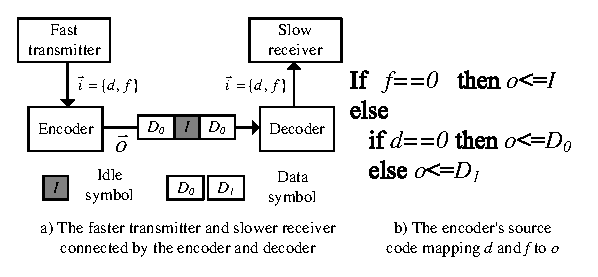
\includegraphics[width=0.5\textwidth]{nonuniq}
\caption{Encoder with flow control mechanism}
\label{fig_fc}
\end{figure}

\begin{figure}[b]
\begin{center}
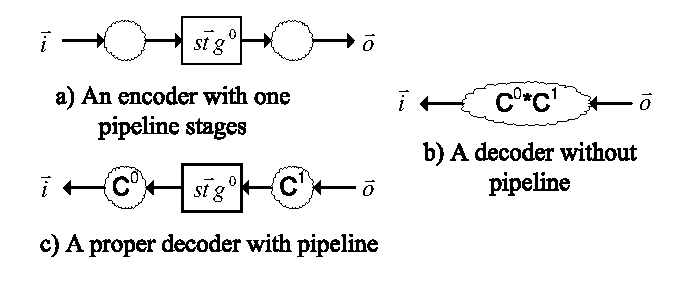
\includegraphics[width=0.4\textwidth]{pipeline}
\end{center}
\caption{The pipelined encoder and its decoders}
\label{fig_pipe}
\end{figure}
% \begin{figure}[b]
% \centering
% 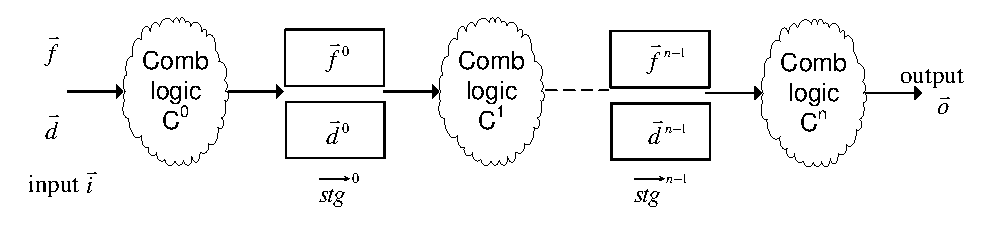
\includegraphics[width=0.5\textwidth]{pipemod1}
% \caption{Encoder with pipeline and flow control mechanism}
% \label{pipemod}
% \end{figure}


Experimental result indicates that this algorithm can always 
generate pipelined decoder with flow control mechanism.

\emph{This paper is organized as follows}.
%Section \ref{sec_casestudy} explains our ideas with a simple example.
Section \ref{sec_prem} introduces the background material;
% Section \ref{sec_findfc} identifies the flow control variables,
% and infers the predicate that enables $\vec{d}$ 
% to be uniquely determined by a bounded sequence of $\vec{o}$;
Section \ref{sec_framework} presents our algorithm framework.
Section \ref{sec_pipeinfer} identifies $\vec{f}^j$ and $\vec{d}^j$ in each pipeline stages $\vec{stg}^j$,
while Section \ref{sec_char} characterizes the decoder's Boolean functions that recover each $\vec{stg}^j$ and the input $\vec{i}$.
Sections \ref{sec_exp} and \ref{sec_relwork} present the experimental results and related works;
Finally,
Section \ref{sec_conclude} sums up the conclusion.

\section{Preliminaries}\label{sec_prem}

% \subsection{Flow control mechanism}\label{subsec_fc}



\subsection{Propositional satisfiability}\label{subsec_SAT}
% We use a denotation similar to that of \cite{TuDAC13}.
The Boolean value set is denoted as $\mathbb{B}=\{0,1\}$.
A vector of variables is represented as $\vec{v}=(v,\dots)$.
$|\vec{v}|$ is the number of variables in $\vec{v}$. 
If a variable $v$ is a member of $\vec{v}$,
then we say $v\in\vec{v}$;
otherwise $v\notin\vec{v}$.
$v\cup\vec{v}$ is a vector that contains both $v$ and all members of $\vec{v}$.
$\vec{v}-v$ is a vector that contains all members of $\vec{v}$ except $v$.
$\vec{a}\cup\vec{b}$ is a vector that contains  all members of $\vec{a}$ and $\vec{b}$.
$\vec{a}-\vec{b}$ is a vector that contains  all members of $\vec{a}$ but no member of $\vec{b}$.

% The set of truth valuations of $\vec{v}$ is denoted as $[\![\vec{v}]\!]$,
% for instance,
% $[\![(v_1,v_2)]\!]=\{(0,0),(0,1),(1,0),(1,1)\}$.

% A Boolean formula $F$ over a variable set $V$ is constructed by connecting variables from $V$ 
% with symbols $\neg$, $\wedge$, $\vee$ and $\Rightarrow$,
% which stand for logical connectives negation, conjunction, disjunction, and implication, respectively.

For formula $F$ over variable set $V$,
SAT solvers try to find a satisfying assignment $A:V\to \mathbb{B}$,
so that $F$ can be evaluated to $1$.
If $A$ exists, then $F$ is satisfiable;
otherwise unsatisfiable.

% A computer program that decides the existence of such a satisfying assignment is called a SAT solver,
%  such as Zchaff\cite{CHAFF},
%  Grasp\cite{grasp},
%  Berkmin\cite{BERKMIN},
%  and MiniSat\cite{EXTSAT}.
 
% Normally,
% a SAT solver requires the formula to be represented in the conjunctive normal form(CNF),
% in which a formula is a conjunction of its clause set,
% and a clause is a disjunction of its literal set,
% and a literal is a variable or its negation.
% A formula in the CNF format is also called a SAT instance,


% \subsection{Cofactoring}\label{subsec_pre_cofact}

% For a Boolean function $f:B^n\to B$,
% we use $supp(f)$ to denote its support set $\{v_1\dots v_n\}$.
% According to \cite{EFFSATUSMCCO},
% the positive and negative cofactors of $f(v_1\dots v\dots v_n)$ with respect to variable
% $v$ are $f_{v\equiv 1}=f(v_1\dots 1\dots v_n)$ and $f_{v\equiv 0}=f(v_1\dots 0\dots v_n)$.
% % respectively.
% % Existential quantification of $f(v_1\dots v\dots v_n)$ with respect to a
% % variable $v$ is $\exists v f=f_v+f_v’$.
% \textbf{Cofactoring} is the action that applies 1 or 0 to $v$ to get $f_{v\equiv 1}$ or $f_{v\equiv 0}$.

% \subsection{Craig interpolation}\label{subsec_pre_interp}
% Craig\cite{Craig} had proved the following theorem:
% \begin{theorem}[Craig Interpolation Theorem\cite{Craig}]\label{thm_craig}
For formulas $\phi_A$ and $\phi_B$,
with $\phi_A\wedge \phi_B$ unsatisfiable,
there exists a formula $\phi_I$ referring only
to the common variables of $\phi_A$ and $\phi_B$ such that $\phi_I\wedge \phi_B$ is unsatisfiable 
and $\phi_A\Rightarrow \phi_I$.
$\phi_I$ is the \textbf{interpolant} \cite{Craig} of $\phi_A$ with respect to $\phi_B$.
% \end{theorem}
% and use McMillan's algorithm \cite{interp_McMillan} to generate it.




\subsection{Finite state machine(FSM)}\label{subsec_fsm}



The encoder is modeled by a FSM $M=(\vec{s},\vec{i},\vec{o},T)$,
consisting of a state variable vector $\vec{s}$,
% an initial state $s_0\in S$,
an input variable vector $\vec{i}$,
% a finite set of configuration letters $C$,
an output variable vector $\vec{o}$,
% and a transition function $T: [\![\vec{s}]\!]\times [\![\vec{i}]\!]\to [\![\vec{s}]\!]\times [\![\vec{o}]\!]$ 
and a transition function $T: \vec{s}\times \vec{i}\to \vec{s}\times \vec{o}$ 
that computes the next state and output variable vector from the current state and input variable vector.
% As shown in Fig. \ref{mealy},
% as well as in the remainder of this paper,
% the state is represented as a gray round corner box,
% and the transition function $T$ is represented as a white rectangle.
When unrolling transition function $T$,
$s\in\vec{s}$,  $i\in\vec{i}$ and  $o\in\vec{o}$ at the $n$-th step 
are respectively denoted as $s_n$, $i_n$ and $o_n$.
% Furthermore,
$\vec{s}$, $\vec{i}$ and $\vec{o}$ at the $n$-th step are respectively denoted as $\vec{s}_n$, $\vec{i}_n$ and $\vec{o}_n$.
% We further denote the sequence of state, input letter and output letter from the $n$-th to the $m$-th step respectively as $s_n^m$, $i_n^m$ and $o_n^m$.
A \textbf{path} is a state sequence $<\vec{s}_n,\dots,\vec{s}_m>$ with $\exists \vec{i}_j\vec{o}_j (\vec{s}_{j+1},\vec{o}_j)\equiv T(\vec{s}_j,\vec{i}_j)$ for all $n\le j< m$.
A \textbf{loop} is a path $<\vec{s}_n,\dots,\vec{s}_m>$ with $\vec{s}_n\equiv \vec{s}_m$.



\subsection{The halting algorithm that determines whether $i\in\vec{f}$}\label{subsec_chkextdec}

\begin{algorithm}[t]
\SetAlgoVlined
\KwIn{The input variable $i\in\vec{i}$.}
% \KwOut{$\vec{f}\subset \vec{i}$, and the maximal $p$, $l$ and $r$ reached.}
% $\vec{f}: = \{\}$;$\vec{d}:= \{\}$;
$p$:= 0 ;~$l$:= 0 ;~$r$:= 0 \;
\ShowLnLabel{while}\While{$true$}{
%   assume $i\in\vec{i}$\;
  $p++$; ~ $l++$; ~ $r++$\;
  \lIf {$Sound(i)$} {
    \ShowLnLabel{adduniq}
\KwRet ($true$, $p$, $l$, $r$)
  }\;\ShowLnLabel{nonuniqres}
  \lElseIf {$Complete(i)$}{
%     $\vec{d}:=i\cup\vec{d}$ ; ~
\KwRet ($false$, $0$, $0$, $0$)
  }
}
\caption{Determine whether $i$ can be uniquely determined by a bounded sequence of $\vec{o}$}
\label{alg_fofc}
\end{algorithm}

\begin{figure}[t]
\begin{center}
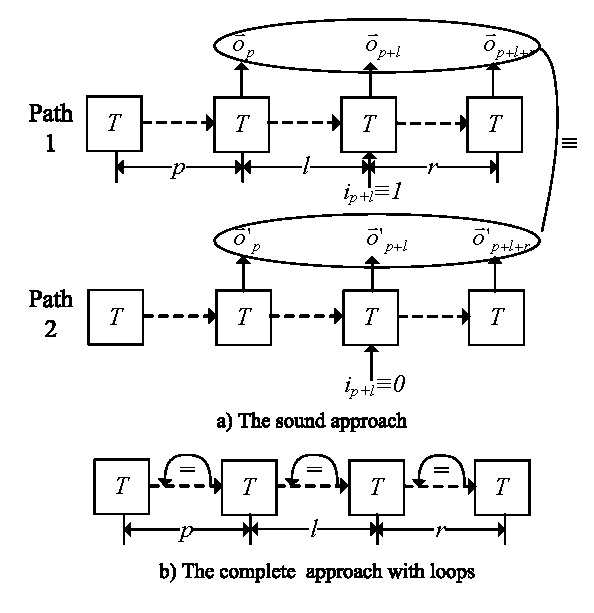
\includegraphics[width=0.4\textwidth]{pc}
\end{center}
\caption{The sound and complete approximative approaches}
  \label{fig_pc}
\end{figure}

Qin et al. \cite{QinTODAES15} proposed Algorithm \ref{alg_fofc}
to determine whether an input variable $i\in\vec{i}$ can be uniquely determined by a bounded sequence of $\vec{o}$,
by iteratively calling 
a sound and a complete approaches until they converge.
% The first one is an under-approximative one that presented in \ref{subsub_sound},
% while the second one is an over-approximative one presented in \ref{subsub_complete}.
% We will present these two approaches below and show 
% that they will eventually converge.

\subsubsection{The sound approach in Fig. \ref{fig_pc}a) shows how to check whether
an input variable $i\in\vec{i}$ can be uniquely determined by a bounded sequence of $\vec{o}$}\label{subsub_sound}
if there exists $p$, $l$ and $r$,
such that for every output sequence $<\vec{o}_p,\dots,\vec{o}_{p+l+r}>$,
$i_{p+l}$ cannot be different.
This is equal to the unsatisfiability of $F_{PC}(p,l,r)$ in Equation (\ref{uniqt1}),
in which Line 1 and 2 of correspond to the two paths in Fig. \ref{fig_pc}a),
Line 3 forces these two paths' output to be the same,
while Line 4 forces their $i_{p+l}$ to be different.
% If there exists such $p$, $l$ and $r$ that can make $F_{PC}(p,l,r)$ unsatisfiable,
% then they can eventually be found by iteratively increasing  $p$, $l$ and $r$,
% and checking for the unsatisfiability of $F_{PC}(p,l,r)$.
% So this approach is sound.


\begin{multline}\label{uniqt1}
%\begin{split}
F_{PC}(p,l,r):= \\
\left\{
\begin{array}{cc}
&\bigwedge_{m=0}^{p+l+r}
\{
(\vec{s}_{m+1},\vec{o}_m)\equiv T(\vec{s}_m,\vec{i}_m)
\}
\\
\wedge&\bigwedge_{m=0}^{p+l+r}
\{
(\vec{s'}_{m+1},\vec{o'}_m)\equiv T(\vec{s'}_m,\vec{i'}_m)
\}
\\
\wedge&\bigwedge_{m=p}^{p+l+r}\vec{o}_m\equiv \vec{o'}_m \\
\wedge& i_{p+l}\equiv 1 \wedge  i'_{p+l}\equiv 0 
% \wedge&\bigwedge_{m=0}^{p+l+r}assertion(\vec{i}_m) \\
% \wedge&\bigwedge_{m=0}^{p+l+r}assertion(\vec{i'}_m) 
\end{array}
\right\}
%\end{split}
\end{multline}




% Here,
% $p$ is the length of the prefix state transition sequence.
% $l$ and $r$ are the lengths of the two output sequences 
% $<\vec{o}_{p+1},\dots,\vec{o}_{p+l}>$ and $<\vec{o}_{p+l+1},\dots,\vec{o}_{p+l+r}>$
% used to determine $i_{p+l}$.

% Line 5 and 6 are the assertion predicates given 
% by the user that constrain the valid valuation on $\vec{i}$.
% PC in $F_{PC}$ is the abbreviation of "parameterized complementary",
% which means $F_{PC}(p,l,r)$ is used to check whether the encoder's input can be uniquely determined with the three parameters $p$, $l$ and $r$.


% According to Fig. \ref{fig_pc}a),
% the first three lines of Equation (\ref{uniqt1}) are two unrolled transition function sequences with the same output sequences.
% They can always be satisfied with the same input variable vectors and initial state vector.
% And the last two lines are constraints on input variable vectors.
% We always check their satisfiability before running our algorithm.
% So the unsatisfiability of $F_{PC}(p,l,r)$ always means $i_{p+l}\equiv i'_{p+l}$.
% 
% 
% % According to Fig. \ref{fig_pc},
% % % it is obvious that,
% % if $F_{PC}(p,l,r)$ is unsatisfiable,
% % then $F_{PC}(p',l',r')$ is also unsatisfiable for $p'\ge p$, $l'\ge l$ and $r'\ge r$.
% According to Equation (\ref{uniqt1}),
% % and Fig. \ref{fig_pc},
% % we can find that,
% for $p'\ge p$, $l'\ge l$ and $r'\ge r$,
% the clause set of $F_{PC}(p',l',r')$ is a super set of $F_{PC}(p,l,r)$.
% % This also lead to the same conclusion.
% % This means,
% So,
% the bounded proof of $F_{PC}(p,l,r)$'s unsatisfiability
% can be generalized to unbounded cases.
% 
% \begin{proposition}\label{prop_pc1}
% If $F_{PC}(p,l,r)$ is unsatisfiable,
% % then $i_{p+l}$ cannot take on two different values for any particular valuation of the output sequence $<\vec{o}_{p},\dots,\vec{o}_{p+l+r}>$,
% then $i_{p+l}$ can be uniquely determined by $<\vec{o}_{p},\dots,\vec{o}_{p+l+r}>$ for all larger $p$, $l$ and $r$.
% \end{proposition}



\subsubsection{The complete approach in Fig. \ref{fig_pc}b) shows how to check whether
an input variable $i\in\vec{i}$ can NOT be uniquely determined by a bounded sequence of $\vec{o}$}\label{subsub_complete}
% For the iterative and sound approach presented in the last subsection,
% if there is no such $p$, $l$ and $r$ than can make $F_{PC}(p,l,r)$ unsatisfiable.
% then it will loop forever.
% So,
% to obtain a halting algorithm,

It is similar to Fig. \ref{fig_pc}a) but with three new constraints to detect loops 
on the three state sequences $<\vec{s}_{0},\dots,\vec{s}_{p}>$, $<\vec{s}_{p+1},\dots,\vec{s}_{p+l}>$ and 
$<\vec{s}_{p+l+1},\dots,\vec{s}_{p+l+r}>$.
It is formally defined as $F_{LN}(p,l,r)$ in Equation (\ref{uniqln}) 
with the last three lines corresponding to the three new constraints.
If $F_{LN}(p,l,r)$ is satisfiable,
then by unrolling the three loops,
we can be sure that any larger  $p$, $l$ and $r$ can also make $F_{LN}(p,l,r)$ and $F_{PC}(p,l,r)$ satisfiable.
% So we can stop increasing $p$, $l$ and $r$.

\begin{multline}\label{uniqln}
% \begin{split}
F_{LN}(p,l,r):=\\
\left\{
\begin{array}{cc}
&F_{PC}(p,l,r)\\
\wedge&\bigvee_{x=0}^{p-1}\bigvee_{y=x+1}^{p} \{\vec{s}_x\equiv \vec{s}_y\wedge \vec{s'}_x\equiv \vec{s'}_y\} \\
\wedge&\bigvee_{x=p+1}^{p+l-1}\bigvee_{y=x+1}^{p+l} \{\vec{s}_x\equiv \vec{s}_y\wedge \vec{s'}_x\equiv \vec{s'}_y\} \\
\wedge&\bigvee_{x=p+l+1}^{p+l+r-1}\bigvee_{y=x+1}^{p+l+r} \{\vec{s}_x\equiv \vec{s}_y\wedge \vec{s'}_x\equiv \vec{s'}_y\}
\end{array}
\right\}
% \end{split}
\end{multline}

Algorithm \ref{alg_fofc} is a halting algorithm because 
if there indeed exists such $p$, $l$ and $r$ that make $F_{PC}(p,l,r)$ unsatisfiable,
then they can eventually be found in Line \ref{adduniq};
Otherwise,
$p$, $l$ and $r$ will eventually be larger than the length of the encoder's longest non-loop path,
which makes $F_{LN}(p,l,r)$ satisfiable.
Both cases will terminate the loop.

% LN in $F_{LN}$ stands for "loop non-complementary",
% which means $F_{LN}(p,l,r)$ with three loops is used to check whether 
% the input variable can NOT be uniquely determined.


% When $F_{LN}(p,l,r)$ is satisfiable,
% then $i_{p+l}$ can't be uniquely determined by $<\vec{o}_{p},\dots,\vec{o}_{p+l+r}>$.
% More importantly,
% by unrolling these three loops,
% we can generalize the satisfiability of $F_{LN}(p,l,r)$ to all larger $p$, $l$ and $r$.
% This means:
% 
% 
% \begin{proposition}\label{prop_ln1}
% If $F_{LN}(p,l,r)$ is satisfiable,
% then $i_{p+l}$ cannot be uniquely determined by $<\vec{o}_{p},\dots,\vec{o}_{p+l+r}>$ for all larger $p$, $l$ and $r$.
% \end{proposition}

% \subsubsection{Identifying flow control vector $\vec{f}$ with Algorithm \ref{alg_fofc}}\label{subsubsec_findfc}
% % To facilitate the presentation of our algorithm,
% % We assume that the input variable vector $\vec{i}$ can be partitioned into 
% % the flow control vector $\vec{f}$ and the data vector $\vec{d}$.
% % The flow control vector $\vec{f}$ is used to indicate the validness of $\vec{d}$.
% % So,
% % for a properly designed encoder,
% % $\vec{f}$ should always be uniquely determined by a bounded sequence of the encoder's output vector $\vec{o}$,
% % or else the decoder cannot recognize the validness of $\vec{d}$.
% % 
% % Thus,
% % Algorithm \ref{alg_fofc} is proposed to identify $\vec{f}$.
% % At Line \ref{initfd},
% % the initial value of $f$ and $d$ are set to empty vector.
% % At Line \ref{initplr},
% % the initial value of $p$, $l$ and $r$ are all set to 0.
% % At Line \ref{while},
% % a while loop is used to iterate on all $i\in\vec{i}$.
% At Line \ref{adduniq},
% the input $i$ that can be uniquely determined will be moved to vector $\vec{f}$.
% % On the other hand,
% If $F_{LN}(p,l,r)$ is satisfiable at Line \ref{nonuniqres},
% the input $i$ that can NOT be uniquely determined will be moved to vector $\vec{d}$.
% Please refer to \cite{QinTODAES15} for its termination and correctness.




% \section{Inferring the flow control predicate $valid(\vec{f})$}


% Furthermore,
% the validness of $\vec{d}$ is indicated by a predicate $valid(\vec{f})$.
% So for a properly designed encoder,
% $valid(\vec{f})$ should make $\vec{d}$ to be uniquely determined by the encoder's output.

% In Subsection \ref{subsec_craig},
% we propose  an algorithm 
% to characterize a Boolean function that makes a Boolean formula satisfiable.
% In Subsection \ref{subsec_infer},
% we apply this algorithm to infer $valid(\vec{f})$,
% % the predicate that enable $\vec{d}$ to be uniquely determined by a bounded sequence of $\vec{o}$.
% the predicate that enables $\vec{d}$ to be uniquely determined.


\subsection{Inferring $valid(\vec{f})$ that makes $\vec{d}$ to be uniquely determined}\label{subsec_infer}

For Boolean relation $R(\vec{a},\vec{b},t)$ with $R(\vec{a},\vec{b},0)\wedge R(\vec{a},\vec{b},1)$ unsatisfiable,
Subsection 4.1 of \cite{QinTODAES15} proposes an algorithm 
to characterize a Boolean function 
that covers exactly all the valuations of $\vec{a}$ 
that can make $R(\vec{a},\vec{b},1)$ satisfiable:
\begin{multline}\label{eq_charsat}
 CharacterizingFormulaSAT(R,\vec{a},\vec{b},t):=\\\{\vec{a}|\exists \vec{b},R(\vec{a},\vec{b},1)~is~satisfiable\}
\end{multline}

% This equation will be used frequently in the remainder of this paper.
Its implementation will not be presented here.

% As shown in Fig. \ref{fig_mono},
Subsection 4.2 of \cite{QinTODAES15} proposed Algorithm \ref{algo_infer} to infer $valid(\vec{f})$ by iteratively increasesing $p$, $l$ and $r$,
and calling $CharacterizingFormulaSAT$ to characterize $Under(p,l,r)$,
a monotonically growing under-approximation of $valid(\vec{f})$,
and $Over(p,l,r)$,
a monotonically shrinking over-approximation of $valid(\vec{f})$.
They will eventually converge to $valid(\vec{f})$.
Please refer to \cite{QinTODAES15} for details.
% 
% \subsubsection{Monotonically growing under-approximation}\label{subsub_nonloop}
% By replacing $i$ in Equation (\ref{uniqt1}) with $\vec{d}$ inferred in Algorithm \ref{alg_fofc},
% and collecting the 3rd line of (\ref{uniqt1}) into Equation (\ref{tpc}):
% 
% 
% 
% \begin{equation}\label{tpc}
% % \begin{split}
% T_{PC}(p,l,r):=\\
% \left\{
% \begin{array}{cc}
%       &\bigwedge_{m=p}^{p+l+r}\vec{o}_m\equiv \vec{o'}_m \\
% \end{array}
% \right\}
% % \end{split}
% \end{equation}
% 
% \begin{figure}[b]
% \begin{center}
% \includegraphics[width=0.4\textwidth]{mono}
% \end{center}
% \caption{The monotonicity of $FSAT_{PC}(p,l,r)$ and $FSAT_{LN}(p,l,r)$}
%   \label{fig_mono}
% \end{figure}
% 
% we have:
% 
% \begin{multline}\label{fpcq}
% % \begin{split}
% F'^d_{PC}(p,l,r,t):=\\
% \left\{
% \begin{array}{cc}
% &\bigwedge_{m=0}^{p+l+r}
% \{
% (\vec{s}_{m+1},\vec{o}_m)\equiv T(\vec{s}_m,\vec{i}_m)
% \}
% \\
% \wedge&\bigwedge_{m=0}^{p+l+r}
% \{
% (\vec{s'}_{m+1},\vec{o'}_m)\equiv T(\vec{s'}_m,\vec{i'}_m)
% \}
% \\
% \wedge& t\equiv T_{PC}(p,l,r)\\
% \wedge& \vec{d}_{p+l}\ne \vec{d'}_{p+l} \\
% % \wedge&\bigwedge_{m=0}^{p+l+r}assertion(\vec{i}_m) \\
% % \wedge&\bigwedge_{m=0}^{p+l+r}assertion(\vec{i'}_m) 
% \end{array}
% \right\}
% % \end{split}
% \end{multline}
% 
% 
% If $F'^d_{PC}(p,l,r,1)$ is satisfiable,
% then $\vec{d}_{p+l}$ can't be uniquely determined by $<\vec{o}_p,\dots,\vec{o}_{p+l+r}>$.
% We further define:
% 
% 
% \begin{multline}\label{pcdef1}
% \begin{array}{l}
% \vec{a}:=  \vec{f}_{p+l}\\
% \vec{b}:= \vec{s}_0\cup \vec{s'}_0\cup\bigcup_{0\le x\le p+l+r}(\vec{i}_{x}\cup\vec{i'}_{x}) - \vec{a}
% % R(\vec{a},\vec{b},t):=  F'^d_{PC}(p,l,r,t)
% \end{array}
% \end{multline}
% 
% 
% Thus,
% as shown in Fig. \ref{fig_pc}a),
% $\vec{a}\cup\vec{b}$ contains all the input variable vectors $\vec{i}_j$ and $\vec{i'}_j$.
% It also contains the two initial states vectors $\vec{s}_0$ and $\vec{s'}_0$.
% So $\vec{a}$ and $\vec{b}$ can uniquely determine the value of $t$ in $F'^d_{PC}(p,l,r,t)$,
% which means $F'^d_{PC}(p,l,r,1)\wedge F'^d_{PC}(p,l,r,0)$ is unsatisfiable.
% Thus,
% the Boolean function over $\vec{f}_{p+l}$ that makes $F'^d_{PC}(p,l,r,1)$ satisfiable can be computed 
% by calling $CharacterizingFormulaSAT$ in Equation (\ref{eq_charsat}) with $F'^d_{PC}(p,l,r,t)$, $\vec{a}$ and $\vec{b}$:
% 
% \begin{multline}\label{fsat_pc}
% FSAT_{PC}(p,l,r):=\\
% CharacterizingFormulaSAT(F'^d_{PC}(p,l,r,t),\vec{a},\vec{b},t)
% \end{multline}
% 
% As shown in Fig. \ref{fig_mono},
% $\neg FSAT_{PC}(p,l,r)$ is an under-approximation of $valid(\vec{f})$ monotonically growing with respect to 
% $p$, $l$ and $r$.
% 
% 
% 
% 
% \subsubsection{Computing monotonically shrinking over-approximation}\label{subsub_loop}
% Similarly,
% we can define :
% 
% \begin{multline}\label{tln}
% % \begin{split}
% T_{LN}(p,l,r):=\\
% \left\{
% \begin{array}{cc}
%       &\bigwedge_{m=p}^{p+l+r}\vec{o}_m\equiv \vec{o'}_m \\
% \wedge&\bigvee_{x=0}^{p-1}\bigvee_{y=x+1}^{p} \{\vec{s}_x\equiv \vec{s}_y\wedge \vec{s'}_x\equiv \vec{s'}_y\} \\
% \wedge&\bigvee_{x=p+1}^{p+l-1}\bigvee_{y=x+1}^{p+l} \{\vec{s}_x\equiv \vec{s}_y\wedge \vec{s'}_x\equiv \vec{s'}_y\} \\
% \wedge&\bigvee_{x=p+l+1}^{p+l+r-1}\bigvee_{y=x+1}^{p+l+r} \{\vec{s}_x\equiv \vec{s}_y\wedge \vec{s'}_x\equiv \vec{s'}_y\}
% \end{array}
% \right\}
% % \end{split}
% \end{multline}
% 
% 
% \begin{multline}\label{lndef1}
% F'^d_{LN}(p,l,r,t):=\\
% \left\{
% \begin{array}{cc}
% &\bigwedge_{m=0}^{p+l+r}
% \{
% (\vec{s}_{m+1},\vec{o}_m)\equiv T(\vec{s}_m,\vec{i}_m)
% \}
% \\
% \wedge&\bigwedge_{m=0}^{p+l+r}
% \{
% (\vec{s'}_{m+1},\vec{o'}_m)\equiv T(\vec{s'}_m,\vec{i'}_m)
% \}
% \\
% % \wedge& \vec{f}_{p+l}\equiv \vec{f'}_{p+l}\\
% \wedge& t\equiv T_{LN}(p,l,r)\\
% \wedge& \vec{d}_{p+l}\ne \vec{d'}_{p+l} \\
% % \wedge&\bigwedge_{m=0}^{p+l+r}assertion(\vec{i}_m) \\
% % \wedge&\bigwedge_{m=0}^{p+l+r}assertion(\vec{i'}_m) 
% \end{array}
% \right\}
% \end{multline}
% 
% 
% \begin{multline}\label{fsat_ln}
% FSAT_{LN}(p,l,r):=\\
% CharacterizingFormulaSAT(F'^d_{LN}(p,l,r,t),\vec{a},\vec{b},t)
% \end{multline}
% 
% As shown in Fig. \ref{fig_mono},
% $\neg FSAT_{LN}(p,l,r)$ is an over-approximation of $valid(\vec{f})$ monotonically shrinking with respect to
% $p$, $l$ and $r$.
% 
% 
% 
% 
% \subsubsection{Inferring $valid(\vec{f})$ with Algorithm \ref{algo_infer}}\label{subsub_overal}
\begin{algorithm}[t]
\SetAlgoVlined
% \KwIn{The Boolean formula $R(\vec{a},\vec{b},t)$, 
% its important variable vector $\vec{a}$,
% its non-important variable vector $\vec{b}$,
% and its target variable $t$.}
% \KwOut{$F_i(\vec{a})$ that makes $R(\vec{a},\vec{b},1)$ satisfiable.}
% $p$:= $0$;~$l$:= $0$;~$r$:= $0$ \;
\While { $Under(p,l,r)\ne Over(p,l,r)$ } {
  $p$ ++ ;~$l$ ++ ;~$r$ ++ \;
}
\KwRet {$Under(p,l,r)$}
\caption{Inferring $valid(\vec{f}_{p+l})$}
\label{algo_infer}
\end{algorithm}

% It just iteratively increases the value of $p$, $l$ and $r$, 
% until $FSAT_{PC}(p,l,r)$ and $FSAT_{LN}(p,l,r)$ converge.
% Please refer to \cite{QinTODAES15} for the proofs of its termination and correctness.




\section{Algorithm Framework}\label{sec_framework}


% \subsection{A general model for the encoder}
As shown in Fig. \ref{fig_pipeenc},
we assume that 
the encoder has $n$ pipeline stages $\vec{stg}^j$,
where $0\le j \le n-1$.
And each pipeline stage $\vec{stg}^j$ can be further partitioned into flow control vector $\vec{f}^j$ and data vector $\vec{d}^j$.
The input vector $\vec{i}$,
as in \cite{QinTODAES15},
can also be partitioned into flow control vector $\vec{f}$ and data vector $\vec{d}$.
If we take the combinational logic block $C^j$ as a function,
then this encoder can be represented by the following equations.

\begin{equation}\label{equ_genpipe}
\begin{array}{cccc}
\vec{stg}^0   & := & C^0(\vec{i})         &\\
\vec{stg}^j   & := & C^j(\vec{stg}^{j-1}) & 1\le j\le n-1\\
\vec{o}       & := & C^n(\vec{stg}^{n-1}) &
\end{array}
\end{equation}


\begin{figure}[b]
\begin{center}
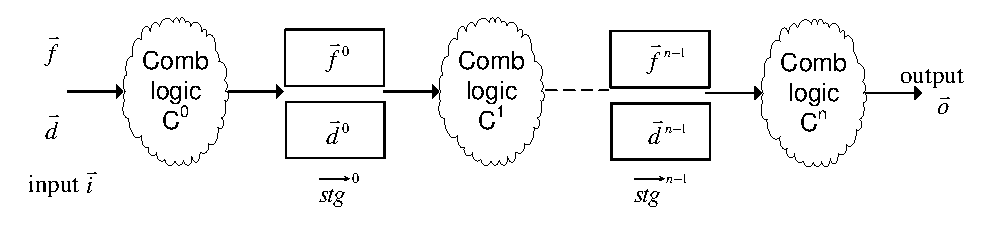
\includegraphics[width=0.5\textwidth]{pipemod1}
\end{center}
\caption{The encoder's general structure with pipeline and flow control}
  \label{fig_pipeenc}
\end{figure}


% Thus,
% each $C^j$ can be seen as a small encoder.
% Assume that $(C^j)^{-1}$ is $C^j$'s decoder function,
% then the pipelined decoder should be like this:
% 
% \begin{equation}\label{equ_genpipedecoder}
% \begin{array}{cccc}
% \vec{stg}^{n-1}       & := & (C^n)^{-1}(\vec{o}) &\\
% \vec{stg}^{j-1}   & := & (C^j)^{-1}(\vec{stg}^j) & 1\le j\le n-1\\
% \vec{i}   & := & (C^0)^{-1}(\vec{stg}^0)         &
% \end{array}
% \end{equation}





% Thus,
% each $C^j$ can be seen as a small encoder that computes $\vec{stg}^j$ or $\vec{o}$
% from $\vec{stg}^{j-1}$ or $\vec{i}$.



% \subsection{Algorithm framework}

With this encoder model,
our algorithm framework is:

\begin{enumerate}
 \item Calling Algorithm \ref{alg_fofc} for each $i\in\vec{i}$ to partition $\vec{i}$ into $\vec{f}$ and $\vec{d}$.
 And defining $(p,l,r)$ to be the maximal one  returned from all calls to Algorithm \ref{alg_fofc}.
 \item Calling Algorithm \ref{algo_infer} to infer $valid(\vec{f})$ that enables $\vec{d}$ 
 to be uniquely determined with parameters $p$, $l$ and $r$.
 \item In Section \ref{sec_pipeinfer}, 
 identifying $\vec{f}^j$ and $\vec{d}^j$ in each pipeline stage $\vec{stg}^j$. 
 \item In Section \ref{sec_char}, 
 characterizing the decoder's Boolean functions that recover each pipeline stages $\vec{stg}^j$
 and input vector $\vec{i}$.
\end{enumerate}



\section{Inferring the encoder's pipeline structure}\label{sec_pipeinfer}

% \subsection{Inferring $p$, $l$ and $r$}\label{subsec_inferplr}
% Before inferring the pipeline stages,
% we first apply the algorithm of \cite{ShenTCAD11} to infer the value of $p$, $l$ and $r$ that can make the 
% output sequence $<o_{p},\dots,o_{p+l+r}>$ uniquely determine all $i_{p+l}\in \vec{i}_{p+l}$.
% This algorithm iteratively increase a parameter $b$,
% and set $p$, $l$ and $r$ all to $b$,
% until $F_{PC}(p,l,r)$ become unsatisfiable for all $i_{p+l}\in \vec{i}_{p+l}$.

\subsection{Minimizing $r$}\label{reduceing}

In the remainder of this paper,
superscript always means the pipeline stage,
while the subscript,
as mentioned in Subsection \ref{subsec_fsm},
always means the step index in the unrolled transition function.
For example,
$\vec{stg}^j$ is the $j$-th pipeline stage.
While $\vec{stg}^j_i$ is the value of this $j$-th pipeline stage 
at the $i$-th step in the unrolled state transition sequence.

With this notation,
we can substitute Equation (\ref{equ_genpipe}) into Fig. \ref{fig_pc}a).
This leads to the following observations,
which is also shown intuitively in Fig. \ref{fig_encexp}:

\begin{enumerate}
\item $\vec{i}_{p+l}$,
the value of input $\vec{i}$ at step $p+l$,
can be uniquely determined by $\vec{stg}^0_{p+l}$,
the value of  the 1st pipeline stage $\vec{stg}^0$ at the same step $p+l$;
 \item $\vec{stg}^0_{p+l}$,
the value of the 1st pipeline stage $\vec{stg}^0$ at step $p+l$,
can be uniquely determine by $\vec{stg}^{1}_{p+l+1}$,
the value of the 2nd pipeline stage $\vec{stg}^{1}$ at the next step $p+l+1$.
 \item ...
 \item $\vec{stg}^{j}_{p+l+j}$,
 the value of $\vec{stg}^{j}$ at step $p+l+j$,
 can be uniquely determine by $\vec{stg}^{j+1}_{p+l+j+1}$,
 the value of next pipeline stage $\vec{stg}^{j+1}$ at the next step $p+l+j+1$.
 \item ...
 \item $\vec{stg}^{r'}_{p+l+r'}$,
 the value of the last pipeline stage $\vec{stg}^{r'}$ at step $p+l+r'$,
 can be uniquely determined by $\vec{o}_{p+l+r'}$,
 the value of output $\vec{o}$ at the same step $p+l+r'$.
\end{enumerate}



\begin{figure}[b]
\begin{center}
\includegraphics[width=0.5\textwidth]{encexp}
\end{center}
\caption{Unrolled transition function with pipeline stages}
  \label{fig_encexp}
\end{figure}

With these observations,
it is obvious that $\vec{i}_{p+l}$ can be uniquely determined by $\vec{o}_{p+l+r'}$.
By comparing this conclusion to Fig. \ref{fig_pc} and Algorithm \ref{alg_fofc},
we can be sure that $r'\le r$.
To find out $r'$, 
we define the following new formula:



% As Algorithm \ref{algo_infer} increases $p$, $l$ and $r$ simultaneously,
% there may be some redundancy in the value of $l$ and $r$.
% So we need to first minimize $r$ in Algorithm \ref{algo_remove2}.



\begin{multline}\label{uniqt11}
% \begin{split}
F'_{PC}(p,l,r'):=\\
\left\{
\begin{array}{cc}
&\bigwedge_{m=0}^{p+l+r'}
\{
(\vec{s}_{m+1},\vec{o}_m)\equiv T(\vec{s}_m,\vec{i}_m)
\}
\\
\wedge&\bigwedge_{m=0}^{p+l+r'}
\{
(\vec{s'}_{m+1},\vec{o'}_m)\equiv T(\vec{s'}_m,\vec{i'}_m)
\}
\\
\wedge&\vec{o}_{p+l+r'}\equiv \vec{o'}_{p+l+r'} \\
\wedge& i_{p}\equiv 1 \wedge  i'_{p}\equiv 0 
% \wedge&\bigwedge_{m=0}^{p+l+r}assertion(\vec{i}_m) \\
% \wedge&\bigwedge_{m=0}^{p+l+r}assertion(\vec{i'}_m) 
\end{array}
\right\}
% \end{split}
\end{multline}


\begin{algorithm}[t]
\SetAlgoVlined
\For{$r':=r \to 0$} {
\ShowLnLabel{testr_1}
  \If{$r'\equiv 0$ or $F'_{PC}(p,l,r'-1)\wedge valid(\vec{f}_{p+l})$ is satisfiable for some $i\in \vec{i}$} {
    break
  }
}
return $r'$
\caption{Minimizing $r$}
\label{algo_remove2}
\end{algorithm}

Compared to Equation (\ref{uniqt1}),
this new formula tries to use only $\vec{o}_{p+l+r'}$ instead of 
sequence $<\vec{o}_{p+l},\dots,\vec{o}_{p+l+r}>$ to uniquely determine $\vec{i}_{p+l}$.

Algorithm \ref{algo_remove2} is proposed to use this new formula to find out $r'$.
% To simplify the presentation,
% we will only introduce the $r$ case.
In Line \ref{testr_1},
it conjugates the inferred flow control predicate $valid(\vec{f})$  with $F'_{PC}(p,l,r'-1)$.
If it is satisfiable,
then $r'$ is the last one that makes $F'_{PC}(p,l,r')\wedge valid(\vec{f}_{p+l})$ unsatisfiable,
we return it directly.
On the other hand,
when $r'\equiv 0$,
$F'_{PC}(p,l,0)$ must have been tested in last iteration,
and the result must be unsatisfiable.
In this case we return $0$.



% Minimizing $l$ is similar but with two exceptions:
% First, 
% the range of $l'$ to be enumerated contains some negative value,
% which means $i$ only depend on the value of $o$ in the future.
% Second,
% to be compatible with such cases,
% we use a new formula $F'_{PC}$ in Line \ref{testr_2}.
% When $l\ge 0$,
% $F'_{PC}$ equals to $F_{PC}$.
% But when $l<0$,
% $F'_{PC}$ is define below:
% 
% \begin{multline}\label{uniqt11}
% % \begin{split}
% F'_{PC}(p,l,r):=\\
% \left\{
% \begin{array}{cc}
% &\bigwedge_{m=0}^{p+l+r}
% \{
% (\vec{s}_{m+1},\vec{o}_m)\equiv T(\vec{s}_m,\vec{i}_m)
% \}
% \\
% \wedge&\bigwedge_{m=0}^{p+l+r}
% \{
% (\vec{s'}_{m+1},\vec{o'}_m)\equiv T(\vec{s'}_m,\vec{i'}_m)
% \}
% \\
% \wedge&\bigwedge_{m=p-l}^{p+r}\vec{o}_m\equiv \vec{o'}_m \\
% \wedge& i_{p}\equiv 1 \wedge  i'_{p}\equiv 0 
% % \wedge&\bigwedge_{m=0}^{p+l+r}assertion(\vec{i}_m) \\
% % \wedge&\bigwedge_{m=0}^{p+l+r}assertion(\vec{i'}_m) 
% \end{array}
% \right\}
% % \end{split}
% \end{multline}
% 
% The only change of Equation (\ref{uniqt11}) compared to Equation (\ref{uniqt1})
% are that 
% the range of output vector is change to $p-l\le m\le p+r$,
% while the subscripts of $i$ and $i'$ in the last line refer to $p$ only,
% $l$ are removed.

% Now, 
% we have a minimized $r$ from Algorithm \ref{algo_remove2},
% which can make $\vec{i}_{p+l}$ to be uniquely determined by $<\vec{o}_{p},\dots,\vec{o}_{p+l+r}>$.
% 
% \begin{figure}[b]
% \begin{center}
% \includegraphics[width=0.25\textwidth]{pc1}
% \end{center}
% \caption{Recovering input with reduced output sequence}
%   \label{fig_pc1}
% \end{figure}
% 
% We further require that :
% \begin{enumerate}
%  \item As shown in Fig. \ref{fig_pc1},
%  $l$ can be reduced to 0,
%  which means $\vec{i}_{p}$ can be uniquely determined by $<\vec{o}_{p},\dots,\vec{o}_{p+r}>$,
%  that is,
%  the set of future outputs.
%  \item The above mentioned output sequence $<\vec{o}_{p},\dots,\vec{o}_{p+r}>$ 
%  can be further reduced to $\vec{o}_{p+r}$.
%  This means $\vec{o}_{p+r}$ is the only output vector needed to recover the input vector $\vec{i}_p$.
% \end{enumerate}
% 
% Checking these two requirements
% equals to checking the unsatisfiability of $F'_{PC}(p,r)\wedge valid(\vec{f}_{p+l})$,
% with $F'_{PC}(p,r)$ defined below:




% This equation seems much stronger than the general requirement in Equation (\ref{uniqt1}).
% But we will show in experimental results that 
% they are always fulfilled.



\subsection{Identifying pipeline stages}\label{subsec_inferstage}

Now,
with $p$ and $l$ inferred by Algorithm \ref{algo_infer} and $r'$ founded by Algorithm \ref{algo_remove2},
we need to generalize $F'_{PC}$ in Equation (\ref{uniqt11}) to the following new formula that
can determine whether $v_j$,
the value of variable $v$ at step $j$
can be uniquely determined by $\vec{w}_k$,
the value of a vector $\vec{w}$ at step $k$.
Now $v_j$ and $\vec{w}_k$ can be either input, state or output variables (vectors).

\begin{multline}\label{uniqt2}
% \begin{split}
F''_{PC}(p,l,r',v_j,\vec{w}_k):=\\
\left\{
\begin{array}{cc}
&\bigwedge_{m=0}^{p+l+r'}
\{
(\vec{s}_{m+1},\vec{o}_m)\equiv T(\vec{s}_m,\vec{i}_m)
\}
\\
\wedge&\bigwedge_{m=0}^{p+l+r'}
\{
(\vec{s'}_{m+1},\vec{o'}_m)\equiv T(\vec{s'}_m,\vec{i'}_m)
\}
\\
\wedge&\vec{w}_{k}\equiv \vec{w'}_{k} \\
\wedge& v_{j}\equiv 1 \wedge  v'_{j}\equiv 0 
% \wedge&\bigwedge_{m=0}^{p+l+r}assertion(\vec{i}_m) \\
% \wedge&\bigwedge_{m=0}^{p+l+r}assertion(\vec{i'}_m) 
\end{array}
\right\}
% \end{split}
\end{multline}

Obviously,
when $F''_{PC}(p,l,r',v_j,\vec{w}_k)$ is unsatisfiable,
$\vec{w}_k$ can uniquely determine $v_j$.

According to Fig. \ref{fig_encexp},
for $0\le j\le r'$,
the flow control vector $\vec{f}^j$ in the $j$-th pipeline stage
is exactly the set of state variables $s\in \vec{s}$ 
that can be uniquely determined at the $p+l+j$-th step by $\vec{o}$ 
at the $p+l+r'$-th step without enforcing $valid(\vec{f}_{p+l})$.
% With Equation (\ref{uniqt2}),
It can be formally defined as:

\begin{equation}\label{stgn_fj}
\vec{f}^{j} := 
 \left\{
 s\in \vec{s} ~| 
\begin{array}{cc}
 F''_{PC}(p,l,r',s_{p+l+j},\vec{o}_{p+l+r'})\\
 ~is~unsatisfiable
\end{array}
\right\}
\end{equation}

% with:
% 
% \begin{equation}\label{stgn_def}
% \begin{array}{ccc}
% % S             & := & \vec{s}/\bigcup_{j<k\le n-2}\vec{stg}^{k}\\
% D             & := & (n-1)-(p+r')\\
% \end{array}
% \end{equation}

While the data vector $\vec{d}^j$ in the $j$-th pipeline stage 
is the set of state variables $s\in \vec{s}$ 
that can be uniquely determined at the same $p+l+j$-th step 
by $\vec{o}$ at the $p+l+r'$-th step with enforcing $valid(\vec{f}_{p+l})$.
% With Equation (\ref{uniqt2}),
It can be formally defined as:

\begin{multline}\label{stgn_dj}
\vec{d}^{j} := \\
 \left\{
 s\in \vec{s} ~| 
 \begin{array}{cc}
 F''_{PC}(p,l,r',s_{p+l+j},\vec{o}_{p+l+r'})\wedge valid(\vec{f}_{p+l})\\
 \wedge valid(\vec{f'}_{p+l})~is~unsatisfiable
 \end{array}
\right\}
\end{multline}

With Equation (\ref{stgn_fj}) and (\ref{stgn_dj}),
pipeline stages can all be identified:

\begin{equation}
 \vec{stg}^j := \vec{d}^j\cup\vec{f}^j
\end{equation}


% Similarly,
% for $0\le j\le n-2$,
% $\vec{f}^j$ at $j-((n-2)-(p+r-1))$-th step
% can be uniquely determined at the $p+r$-th step by $\vec{o}$ without enforcing $valid(\vec{f})$.
% So we can recursively defined $\vec{f}^j$ as :
% 
% \begin{equation}\label{stgn_def}
% \begin{array}{ccc}
% S             & := & \vec{s}/\bigcup_{j<k\le n-2}\vec{stg}^{k}\\
% D             & := & (n-2)-(p+r-1)\\
% \end{array}
% \end{equation}
% 
% \begin{equation}\label{stgn_j}
% \vec{stg}^{j} := 
%  \left\{
%  s\in S ~| 
% % \begin{array}{cc}
%  F''_{PC}(p,r,s,j-D,\vec{stg}^{j+1},j-D+1)
%  ~is~unsatisfiable
% % \end{array}
% \right\}
% \end{equation}
% 
% With Equation (\ref{stgn_1}) and (\ref{stgn_j}),
% all the pipeline stages can now be inferred.

% \subsection{Inferring the pipeline stage that uniquely determines input vector}\label{subsec_inferinput}
% 
% According to Fig. \ref{fig_pipeenc},
% $\vec{stg}^0$ defined in Equation (\ref{stgn_j}) is
% exactly the pipeline stage that uniquely determined the input vector $\vec{i}$.
% 
% But in real encoders,
% this may not be the case.
% So we need to search for the smallest $j$ from $0$ to $n-1$ that can make $\vec{i}$ to be uniquely determined by $\vec{stg}^j$,
% that is,
% the smallest $j$ that can make $F''_{PC}(p,r,i,p,\vec{stg}^{j},j-D)$ unsatisfiable for all $i\in \vec{i}$,
% with $D$ defined in Equation (\ref{stgn_def}).

% \subsection{Finding out the flow control vectors in each pipeline stage}

\section{Characterizing the Boolean functions recovering input variables and pipeline stages}\label{sec_char}
\subsection{Characterizing the Boolean functions recovering the last pipeline stage $\vec{stg}^{r'}$}

According to Equation (\ref{stgn_fj}),
every state variable $s\in \vec{f}^{r'}$ at the $p+l+r'$-th step can be uniquely determined by $\vec{o}_{p+l+r'}$.
That is,
$F''_{PC}(p,l,r',s_{p+l+r'},\vec{o}_{p+l+r'})$ is unsatisfiable and can be partitioned into :

\begin{equation}
 \phi_A := 
 \left\{
\begin{array}{cc}
&\bigwedge_{m=0}^{p+l+r'}
\{
(\vec{s}_{m+1},\vec{o}_m)\equiv T(\vec{s}_m,\vec{i}_m)
\}
\\
\wedge& s_{p+l+r'}\equiv 1 
\end{array}
\right\}
\end{equation}

\begin{equation}
% \begin{split}
\phi_B := 
\left\{
\begin{array}{cc}
&\bigwedge_{m=0}^{p+l+r'}
\{
(\vec{s'}_{m+1},\vec{o'}_m)\equiv T(\vec{s'}_m,\vec{i'}_m)
\}
\\
\wedge&\vec{o}_{p+l+r'}\equiv \vec{o'}_{p+l+r'} \\
\wedge& s'_{p+l+r'}\equiv 0 
% \wedge&\bigwedge_{m=0}^{p+l+r}assertion(\vec{i}_m) \\
% \wedge&\bigwedge_{m=0}^{p+l+r}assertion(\vec{i'}_m) 
\end{array}
\right\}
% \end{split}
\end{equation}

% As $F''_{PC}(p,r,s,p+r,\vec{o},p+r)$ equals to $\phi_A \wedge \phi_B$,
% so $\phi_A \wedge \phi_B$ is unsatisfiable.
% And the common variables of $\phi_A$ and $\phi_B$ is $\vec{o}_{p+l+r'}$.

According to \cite{InterpBoolFunction},
a Craig interpolant $\phi_I$ of $\phi_A$ with respect to $\phi_B$ can be constructed,
which refer only to $\vec{o}_{p+l+r'}$,
the common variables of $\phi_A$ and $\phi_B$.
And $\phi_I$ covers all the valuations of $\vec{o}_{p+l+r'}$ that can make $s_{p+l+r'}\equiv 1$.
At the same time,
$\phi_I\wedge \phi_B$ is unsatisfiable,
which means $\phi_I$ covers nothing that can make $s_{p+l+r'}\equiv 0$.

Thus,
$\phi_I$ can be used as the decoder's Boolean function 
that recovers $s\in \vec{f}^{r'}$ from $\vec{o}$.

According to Algorithm \ref{algo_infer},
the inferred flow control predicate $valid(\vec{f}_{p+l})$ can
enable $\vec{d}_{p+l}$ to be uniquely determined by $\vec{o}_{p+l+r'}$.
By further referring to Fig. \ref{fig_encexp},
this predicate $valid(\vec{f}_{p+l})$ can also enable $\vec{d}^{r'}_{p+l+r'}$ 
in the last pipeline stage to be uniquely determined by output $\vec{o}_{p+l+r'}$.
So,
for each $s\in \vec{d}^{r'}$,
the formula $F''_{PC}(p,l,r',s_{p+l+r'},\vec{o}_{p+l+r'})\wedge valid(\vec{f}_{p+l})\wedge valid(\vec{f'}_{p+l})$ is unsatisfiable 
and can be partitioned into :

\begin{equation}\label{eqn_char_dlast_A}
 \phi_A := 
 \left\{
\begin{array}{cc}
&\bigwedge_{m=0}^{p+l+r'}
\{
(\vec{s}_{m+1},\vec{o}_m)\equiv T(\vec{s}_m,\vec{i}_m)
\}
\\
\wedge& s_{p+l+r'}\equiv 1 \\
\wedge& valid(\vec{f}_{p+l})
\end{array}
\right\}
\end{equation}

\begin{equation}\label{eqn_char_dlast_B}
% \begin{split}
\phi_B := 
\left\{
\begin{array}{cc}
&\bigwedge_{m=0}^{p+l+r'}
\{
(\vec{s'}_{m+1},\vec{o'}_m)\equiv T(\vec{s'}_m,\vec{i'}_m)
\}
\\
\wedge&\vec{o}_{p+l+r'}\equiv \vec{o'}_{p+l+r'} \\
\wedge& s'_{p+l+r'}\equiv 0 \\
\wedge& valid(\vec{f'}_{p+l})
% \wedge&\bigwedge_{m=0}^{p+l+r}assertion(\vec{i}_m) \\
% \wedge&\bigwedge_{m=0}^{p+l+r}assertion(\vec{i'}_m) 
\end{array}
\right\}
% \end{split}
\end{equation}


\subsection{Characterizing the Boolean functions recovering other pipeline stages $\vec{stg}^j$}
According to Fig. \ref{fig_encexp},
% Similar to last subsection,
$\vec{f}^j_{p+l+j}$ can be uniquely determined by $\vec{stg}^{j+1}_{p+l+j+1}$.
So for every $s\in\vec{f}^j$,
we can partition the unsatisfiable formula $F''_{PC}(p,l,r',s_{p+l+j},\vec{stg}^{j+1}_{p+l+j+1})$ 
 into:

\begin{equation}
 \phi_A := 
 \left\{
\begin{array}{cc}
&\bigwedge_{m=0}^{p+l+r'}
\{
(\vec{s}_{m+1},\vec{o}_m)\equiv T(\vec{s}_m,\vec{i}_m)
\}
\\
\wedge& s_{p+l+j}\equiv 1 
\end{array}
\right\}
\end{equation}

\begin{equation}
% \begin{split}
\phi_B := 
\left\{
\begin{array}{cc}
&\bigwedge_{m=0}^{p+l+r'}
\{
(\vec{s'}_{m+1},\vec{o'}_m)\equiv T(\vec{s'}_m,\vec{i'}_m)
\}
\\
\wedge&\vec{stg}^{j+1}_{p+l+j+1}\equiv \vec{stg'}^{j+1}_{p+l+j+1} \\
\wedge& s'_{p+l+j}\equiv 0 
% \wedge&\bigwedge_{m=0}^{p+l+r}assertion(\vec{i}_m) \\
% \wedge&\bigwedge_{m=0}^{p+l+r}assertion(\vec{i'}_m) 
\end{array}
\right\}
% \end{split}
\end{equation}

Again,
a Craig interpolant $\phi_I$ of $\phi_A$ with respect to $\phi_B$ can be constructed,
and used as the decoder's Boolean function that recovers $s\in\vec{f}^{j}$ from $\vec{stg}^{j+1}$.

Similar to Equation (\ref{eqn_char_dlast_A}) and (\ref{eqn_char_dlast_B}),
by replacing $F''_{PC}(p,l,r',s_{p+l+j},\vec{stg}^{j+1}_{p+l+j+1})$  with 
$F''_{PC}(p,l,r',s_{p+l+j},\vec{stg}^{j+1}_{p+l+j+1})\wedge valid(\vec{f}_{p+l})\wedge valid(\vec{f'}_{p+l})$ ,
we can characterize the Boolean function that recovers each $s\in\vec{d}^{j}$ from $\vec{stg}^{j+1}$.

\subsection{Characterizing the Boolean functions recovering the encoder's input variables}

According to Fig. \ref{fig_encexp},
$\vec{f}_{p+l}$ can be uniquely determined by the 1st pipeline stage $\vec{stg}^0_{p+l}$.
So for every flow control input $i\in\vec{f}$,
$F''_{PC}(p,l,r',i_{p+l},\vec{stg}^0_{p+l})$ is unsatisfiable and can be partitioned into :

\begin{equation}
% \begin{split}
\phi_A:=
\left\{
\begin{array}{cc}
&\bigwedge_{m=0}^{p+l+r'}
\{
(\vec{s}_{m+1},\vec{o}_m)\equiv T(\vec{s}_m,\vec{i}_m)
\}
\\
\wedge& i_{p+l}\equiv 1 
% \wedge&\bigwedge_{m=0}^{p+l+r}assertion(\vec{i}_m) \\
% \wedge&\bigwedge_{m=0}^{p+l+r}assertion(\vec{i'}_m) 
\end{array}
\right\}
% \end{split}
\end{equation}

\begin{equation}
% \begin{split}
\phi_B:=
\left\{
\begin{array}{cc}
&\bigwedge_{m=0}^{p+l+r'}
\{
(\vec{s'}_{m+1},\vec{o'}_m)\equiv T(\vec{s'}_m,\vec{i'}_m)
\}
\\
\wedge&\vec{stg}^0_{p+l}\equiv \vec{stg'}^0_{p+l} \\
\wedge& i'_{p+l}\equiv 0 
% \wedge&\bigwedge_{m=0}^{p+l+r}assertion(\vec{i}_m) \\
% \wedge&\bigwedge_{m=0}^{p+l+r}assertion(\vec{i'}_m) 
\end{array}
\right\}
% \end{split}
\end{equation}

Again,
the Craig interpolant $\phi_I$ of $\phi_A$ with respect to $\phi_B$ 
can be used as the decoder's Boolean function that recovers $i\in\vec{f}$ from $\vec{stg}^0$.

Similar to Equation (\ref{eqn_char_dlast_A}) and (\ref{eqn_char_dlast_B}),
by replacing $F''_{PC}(p,l,r',i_{p+l},\vec{stg}^0_{p+l})$ with $F''_{PC}(p,l,r',i_{p+l},\vec{stg}^0_{p+l})\wedge valid(\vec{f}_{p+l})\wedge valid(\vec{f'}_{p+l})$,
we can characterize the Boolean function that recovers each $i\in\vec{d}$ from $\vec{stg}^0$.



\section{Experimental results}\label{sec_exp}
We have implemented these algorithms in OCaml language,
and solved the generated CNF formulas with MiniSat 1.14 \cite{EXTSAT}.
All experiments have been run on a server with 16 Intel Xeon E5648 processors at 2.67GHz, 
192GB memory, and CentOS 5.4 Linux.
% All these experimental results and programs can be downloaded 
% from https://github.com/shengyushen/compsyn.

% \subsection{Benchmarks}
%  shows all benchmarks used in this paper.
% They come from \cite{ShenTCAD12}.
%  \item The benchmark package sent to us by Liu, the author of \cite{LiuTCAD12}.
%  So there may be some overlap between (2) and (3).
% \end{enumerate}

\subsection{Comparing timing and area}
We use the benchmarks from Qin et al. \cite{QinTODAES15},
whose experimental results are shown in Table \ref{tab_bench}.
pcie is a PCI Express \cite{pcie} encoder,
while xgxs and t2eth are two Ethernet \cite{IEEE8023_S4} encoders.

The 2nd and 3rd column of Table \ref{tab_bench} show respectively the number of inputs, outputs and registers of each benchmark.
The 4th column shows the area of the encoder when mapped to LSI10K library with Design Compiler.
% We use Design compiler here instead of ABC \cite{ABC} used by other researchers 
% because ABC can not read in verilog files with registers generated by our algorithms.
In this paper, 
all area and delay are obtained in the same setting.
% we can compare them to that of \cite{LiuTCAD12}.



\begin{table}[b]
\caption{Benchmarks and experimental results}
\centering
\begin{tabular}{|c|c|c|c|c|c|c|c|c|c|}
\hline
 Names     & \multicolumn{3}{|c|}{The encoders}                                  &   \multicolumn{3}{|c|}{decoder gener-}             &   \multicolumn{3}{|c|}{decoder gener-} \\    
           & \multicolumn{3}{|c|}{}                                              &   \multicolumn{3}{|c|}{ated by \cite{ShenTCAD11}}  &   \multicolumn{3}{|c|}{ated by this paper} \\\cline{2-10}
           &    \#   &   \#    &area                                             &run  &delay&area                                     &run  &delay&area \\
           & in/out  &  reg    &                                                 &time &(ns) &                                        &time &(ns) &    \\\hline\hline
 pcie      & 10/11   & 23      & 326                                             &0.37 &7.20 &624                                     &8.08 & 5.89&652 \\\hline
 xgxs      & 10/10   & 16      & 453                                             &0.21 &7.02 &540                                     &4.25 & 5.93&829 \\\hline
 t2eth     & 14/14   & 49      & 2252                                            &12.7 &6.54 &434                                     &430.4& 6.12&877 \\\hline
% scrambler  &64/64    & 58      & 1034 & inserting 01 flipping                    &     \multicolumn{6}{|c|}{no pipeline }\\\cline{1-5}
%  xfi       & 72/66   & 72      & 7772 &     Ethernet clause 49 \cite{IEEE8023_S4}&     \multicolumn{6}{|c|}{stages found}\\\hline
\end{tabular}\label{tab_bench}
\end{table}


% \begin{table}[t]
% \caption{Experimental results}
% \begin{tabular}{|c|c|c|c|c|c|c|c|}
% \hline
%            
%  Na-       
%  mes       
%            
%  pcie      &0.37 &7.20 &624 &3.57 & 5.89&652 &9/12\\\hline
%  xgxs      &0.21 &7.02 &540 &1.57 & 5.93&829 &13\\\hline
%  t2eth     &12.7 &6.54 &434 &47.2 & 6.12&877 &8/8/10/20\\\hline
%  scr.      &     \multicolumn{7}{|c|}{no pipeline }\\\cline{1-1}
%  xfi       &     \multicolumn{7}{|c|}{structure found}\\\hline
% \end{tabular}\label{tab_res}
% \end{table}


% Table \ref{tab_res} compares the old algorithm from \cite{ShenTCAD11} to this paper's algorithm.
The 5th to 7th columns show respectively the run time of \cite{ShenTCAD11}'s algorithm to generate the decoder without pipeline,
and the delay and area of the generated decoder.
While the 8th to 10th columns show respectively the run time of this paper's algorithm to generate the pipelined decoder,
and the delay and area of the generated decoder.
% The last column shows the number of registers in each pipeline stage.

Comparing the 6th and the 9th column indicates that
the decoders' delay have been significantly improved.
% And the the last column shows that there actually exist very deep pipeline,
% especially the t2eth with 4 pipeline stages.

% One thing that is a little bit surprise is,
% the two largest benchmarks scrambler and xfi do not have pipeline stages inside.
% We study their code and confirm that this is true.
% Their area are so large because they use much wider datapaths with 64 to 72 bits.
% Please refer to IEEE 802.3ae clause 49 \cite{IEEE8023_S4}  for more details.

\subsection{Inferred pipeline stages of pcie}

The benchmark pcie has two pipeline stages,
whose flow control vector and data vector are respectively shown in Table \ref{tab_pcie}.
The inferred $valid(\vec{f})$ is $CNTL\_TXEnable\_P0$.

\begin{table}[t]
\centering
\caption{Inferred pipeline stages of pcie}
\begin{tabular}{|c|c|c|c|}
\hline
                       & input                  & pipeline stage 0          &  pipeline stage 1    \\\hline\hline
$\vec{f}$ or           &CNTL\_TXEnable\_P0      & InputDataEnable\_P0       & OutputData\_P0[9:0]\\
$\vec{f}^j$            &                        &                           & OutputElecIdle\_P0 \\\hline
% flow control           &CNTL\_TXEnable\_P0      & InputDataEnable\_P0\_reg  & true \\
% predicate              &                        &                           &  \\\hline
$\vec{d}$ or           &TXDATA[7:0]             & InputData\_P0[7:0]        & \\
$\vec{d}^j$              &TXDATAK                 & InputDataK\_P0            & \\\hline
\end{tabular}\label{tab_pcie}
\end{table}


One issue to be noticed that is the data vector at pipeline stage 1 is empty,
while all registers in that stages are recognized as flow control vector.
We inspect the encoder's source code and find that these registers are 
directly fed to output.
So they can actually be uniquely determined by $\vec{o}$.
This doesn't affect the correctness of the generated decoder,
because the functionality of flow control vector never depend on the inferred flow control predicate.


\subsection{Inferred pipeline stages of xgxs}


The benchmark xgxs has only 1 pipeline stage,
whose flow control vector and data vector are respectively shown in Table \ref{tab_xgxs}.
The inferred $valid(\vec{f})$ is $!bad\_code$.

\begin{table}[b]
\centering
\caption{Inferred pipeline stages of xgxs}
\begin{tabular}{|c|c|c|}
\hline
                       & input                  &  pipeline stage 0    \\\hline\hline
$\vec{f}$ or $\vec{f}^j$&bad\_code              & bad\_code\_reg\\\hline
% flow control predicate &!bad\_code              & !bad\_code\_reg\_reg \\\hline
$\vec{d}$ or $\vec{d}^j$&encode\_data\_in[7:0]  &ip\_data\_latch[2:0] \\
                       &konstant                &plus34\_latch     \\
                       &                        &data\_out\_latch[5:0]\\
                       &                        &konstant\_latch   \\
                       &                        &kx\_latch         \\
                       &                        &minus34b\_latch   \\\hline
\end{tabular}\label{tab_xgxs} 
\end{table}


\subsection{Inferred pipeline stages of t2ether}


\begin{table}[t]
\centering
\caption{Inferred pipeline stages of t2ether}
\begin{tabular}{|c|c|c|c|}
\hline
                       & input                        & pipeline                  &  pipeline          \\
                       &                              & stage 0                   &  stage 1           \\\hline\hline
$\vec{f}$ or $\vec{f}^j$& tx\_enc\_ctrl\_sel[3:0]     &qout\_reg\_0\_8            & qout\_reg\_0\_9    \\
                       &                              &qout\_reg\_2\_4            & qout\_reg\_1\_5    \\
                       &                              &qout\_reg\_1\_4            & qout\_reg\_2\_5    \\
                       &                              &                           & qout\_reg\_0\_10   \\\hline
$\vec{d}$ or $\vec{d}^j$&txd[7:0]                     &qout\_reg[7:0]             &qout\_reg[7:0]\_1   \\\hline\hline
                       &  pipeline                    &  \multicolumn{2}{|c|}{pipeline}                \\
                       &  stage 2                     &  \multicolumn{2}{|c|}{stage 3}                 \\\hline\hline
$\vec{f}$ or $\vec{f}^j$&qout\_reg[9:0]\_2            &qout\_reg[7:1]\_3 &qout\_reg\_0\_7              \\
                       &                              &qout\_reg\_8\_1   &sync1\_reg1                  \\
                       &                              &qout\_reg\_9\_1   &sync1\_reg                   \\
                       &                              &qout\_reg\_3\_4   &Q\_reg1                      \\
                       &                              &qout\_reg\_0\_4   &Q\_reg                       \\
                       &                              &qout\_reg\_3\_5   &                             \\\hline
$\vec{d}$ or $\vec{d}^j$&                             &\multicolumn{2}{|c|}{}                          \\\hline
\end{tabular}\label{tab_t2ether}
\end{table}


The benchmark t2ether has four pipeline stages shown in Table \ref{tab_t2ether}.
% The control flow predicates are fairly complex, 
% so we list them below instead of in Table \ref{tab_t2ether}.
The inferred $valid(\vec{f})$ is:
\begin{multline}
\begin{array}{l}
( tx\_enc\_ctrl\_sel[2]~\&~tx\_enc\_ctrl\_sel[3]~)~| \\
( tx\_enc\_ctrl\_sel[2]~\&~!tx\_enc\_ctrl\_sel[3]~\& \\!tx\_enc\_ctrl\_sel[0]~\&~tx\_enc\_ctrl\_sel[1]~)~| \\
( !tx\_enc\_ctrl\_sel[2]~\&~tx\_enc\_ctrl\_sel[3]~)~| \\
( !tx\_enc\_ctrl\_sel[2]~\&~!tx\_enc\_ctrl\_sel[3]~\& \\~tx\_enc\_ctrl\_sel[0] )
\end{array}
\end{multline}

% The flow control predicate $valid(\vec{f}^0)$ for the 0-th pipeline stage is :
% \begin{multline}
% \begin{array}{l}
% ( qout\_reg\_2\_4~\&~qout\_reg\_1\_4~\&~!qout\_reg\_0\_8) | \\
% ( !qout\_reg\_2\_4~\&~qout\_reg\_0\_8)
% \end{array}
% \end{multline}
% 
% The flow control predicate $valid(\vec{f}^1)$ for the 1-th pipeline stage is :
% 
% \begin{multline}
% \begin{array}{l}
% ( qout\_reg\_2\_5~\&~qout\_reg\_1\_5~\&~qout\_reg\_0\_10~\&~!qout\_reg\_0\_9) | \\
% ( qout\_reg\_2\_5~\&~qout\_reg\_1\_5~\&~!qout\_reg\_0\_10) | \\
% ( qout\_reg\_2\_5~\&~!qout\_reg\_1\_5~\&~!qout\_reg\_0\_10) | \\
% ( !qout\_reg\_2\_5~\&~qout\_reg\_0\_10~\&~qout\_reg\_0\_9) | \\
% ( !qout\_reg\_2\_5~\&~!qout\_reg\_0\_10)
% \end{array}
% \end{multline}
% 
% 
% The flow control predicates $valid(\vec{f}^2)$ and $valid(\vec{f}^3)$ for the last two pipeline stages are all $true$.















 















\section{RELATED PUBLICATIONS}\label{sec_relwork}
%\subsection{Complementary Synthesis}
%%Complementary synthesis is an emerging new research topic,
%%there are only two papers that discuss this problem.
%
%The concept of complementary synthesis was first proposed by us\cite{ShengYuShen:iccad09} in ICCAD 2009.
%Its major shortcomings are that it is incomplete,
%and its run-time overhead of building decoder is too large.
%
%The incomplete problem has been addressed by \cite{ShengYuShen:fmcad10}, while \cite{ShengYuShen:tcad} addresses the second shortcoming by simplifying the SAT instance with unsatisfiable core extraction before building decoders.

%\subsection{Complementary synthesis}\label{subsec_compsyn_relat}
Shen et al.\cite{ShenICCAD09} proposed the first complementary synthesis algorithm.
It checks the decoder's existence by iteratively increasing the length of unrolled transition function sequence,
and generates the decoder's Boolean functions by enumerating all satisfying assignments of the decoder's output.
Its major shortcomings are that it may not halt and it is too slow
in building the decoder.

Shen et al.\cite{ShenTCAD11} and Liu et al.\cite{LiuICCAD11} tackled the halting problem independently by searching for loops in the state sequence,
while the runtime overhead problem was addressed in \cite{ShenTCAD12,LiuICCAD11} by Craig interpolant\cite{Craig}.

Shen et al.\cite{ShenTCAD12} automatically inferred an assertion for configuration pins, 
which can lead to the decoder's existence.
% It can be seen as a special case of Algorithm \ref{algo_pcln} in Section \ref{sec_infer},
% with the restriction that the inferred assertion must hold on all cycles,
% to prevent the encoder from leaving the unique state set.

Tu and Jiang \cite{TuDAC13} proposed a break-through algorithm 
that recover the encoder's input by considering its initial and reachable states.

Qin et al. \cite{QinTODAES15}
proposed the first algorithm that can handle encoder with flow control mechanism.
But it can not handle pipeline stages.


% based on property directed reachability analysis\cite{BradleyVMCAI11,EenFMCAD11} 
% that can take the encoder's initial state into consideration,
% so that the infinite history of the encoder and the decoder can be used to generate the decoder's output.
% This algorithm can handle some special encoders that cannot be handled by the state-of-the-art algorithms.
% But for the encoders with flow control mechanism used in our experiments,
% our algorithm is enough, 
% and therefore we have not implemented their algorithm in our framework.

%
%\subsection{Program inversion}\label{subsec_proinv}
%According to Gulwani \cite{dim_syn},
%program inversion involves deriving a program $P^{-1}$
%that negates the computation of a given program $P$.
%So,
%the definition of program inversion is very similar to complementary synthesis.
%
%The initial work on deriving program inversion used proof-based approaches\cite{prog_inv},
%which could handle only very small programs and very simple syntax structures.
%
%Gl\"{u}ck et al. \cite{mtd_autoProginv} inverted first-order functional programs
%by eliminating nondeterminism with LR-based parsing methods.
%But,
%the use of functional languages in that work is incompatible with our complementary synthesis.
%
%Srivastava et al. \cite{prog_inv_rev,program_inversion_11} assumed that an inverse program was typically related to the original program,
%and so the space of possible inversions can be inferred by automatically
%mining the original program for expressions, predicates, and control flow.
%This is somewhat similar to our approach in inferring the pipeline stages.
%This algorithm inductively rules out invalid paths that cannot fulfill the requirement of inversion
%to narrow down the space of candidate programs until only the valid ones remain.
% So,
% it can only guarantee the existence of a solution,
% but not the correctness of this solution if its assumptions do not hold.

% \subsection{The completeness of bounded model checking}\label{subsec_bmc_relate}
% Bounded model checking(BMC) \cite{bmc_tacas99} is a model checking technology that considers only paths of limited length.
% So it is an incomplete algorithm.
% Many researchers have tried to find complete approaches for BMC.
% 
% One line of research\cite{bmc_tacas99,RecDiam} tried to find out a bound $b$,
% which can guarantee the correctness of a specification,
% if the specification is correct on all paths that are shorter than $b$.
% Line 8 of Algorithm \ref{algo_pcln} finds out the value of $p$,$d$ and $l$ that can prove the non-existence of the decoder,
% which is similar to \cite{bmc_tacas99,RecDiam}.
% 
% The other line of research\cite{kind_tacas99} tried to find a bound for induction,
% such that the correctness of a specification within any bound $b$ implies the correctness on bound $b+1$.
% Our algorithm proves the non-existence of the decoder by unfolding loops.
% This is similar to finding induction patterns \cite{kind_tacas99}.

% \textbf{This paper achieves completeness without following these two approaches.
% Instead,
% it defines two complement uniqueness conditions,
% $LP$ and $LL$,
% and find out proper algorithms to check them.}

%\subsection{Temporal Logic Synthesis}
%%Automatically synthesis of program from logic specification is first identified as Church's problem in 1962\cite{LOGARTHAUTO}.
%%Some early researches \cite{SLVSQFSS,AUTOINF} solve this problem by reducing it to checking emptiness of tree automata.
%
%The temporal logic synthesis was first addressed by Clarke et al.\cite{DSGSYNTMPLG} and Manna et al. \cite{SYNTMPLGSPC}.
%But Pnueli et al. \cite{SYNRCTVMD} pointed out that the complexity of LTL synthesis is double exponent.
%%This high complexity drives researchers turning their focus to find smaller but still useful subset of temporal logic,
%%such that synthesis problem can be solved with lower complexity.
%
%One line of research \cite{CNTLSYNTMDAUTO,DTMGENGMELTL,SYNRCTVDES} focuses on the so-called generalized reactive formulas of the form:
%$(\square \lozenge p_1 \wedge \cdots \square \lozenge p_m) \to (\square \lozenge q_1 \wedge \cdots \square \lozenge q_n)$.
%Complexity of solving synthesis problem for such formula is $O(N^3)$.
%
%The other line of research focuses on finding efficient algorithm \cite{SYNCNTLBNDRPN}
%for expensive safra determination algorithm \cite{CMPLXAUTO} on an useful formula subset,
%or just avoiding it\cite{NEWALGSTRGSYN}.
%
%%Yet another approach is antichain\cite{ANTICHAIN},
%%which reduces the expensive state set computation to computation on maximal and minimal elements of lattice.
%
%Based on these research works,
%some tools\cite{ANZU} that can handle small temporal formulas have been developed.
%
%All these works assume a hostile environment,
%which seems too restrictive for many applications.
%So Fisman et al. \cite{rationalsyn_tacas10}, Chatterjee et al. \cite{assguasyn_tacas07} and Ummels et al. \cite{ralgame_istta06} proposed rational synthesis algorithm,
%which assumes that each agents act to achieve their own goals instead of failing each other.


% \subsection{Protocol converter synthesis}
% Protocol converter synthesis is a process that automatically generates a translator between two different communication protocols.
% This is relevant to our work,
% because both focus on synthesizing communication circuits.
% 
% Avnit et al. \cite{converter_date08,converter_todeas09} first defined a general model for describing different protocols,
% and then provided an algorithm to decide
% whether there is some functionality of a protocol that cannot be translated into another.
% Finally,
% they synthesized a translator by computing the greatest fixed point for the update function of the buffer's control states.
% Latter, 
% they \cite{converter_date09} improved their algorithm with a more efficient design space exploration algorithm.


\section{Conclusions}\label{sec_conclude}
This paper proposes the first complementary synthesis algorithm that
can handle encoders with pipeline stages and flow control mechanism.
Experimental result indicates that the proposed algorithm can always 
correctly generate pipelined decoder with flow control mechanism.


% \section*{Acknowledgment}
% The authors would like to thank the anonymous reviewers for their hard work.

% This work was funded by Projects 60603088 and 61070132 supported by National Natural Science Foundation of China.


% \bibliographystyle{abbrv}
% \bibliography{ssy}

% use section* for acknowledgment
% \section*{Acknowledgment}
% 
% 
% The authors would like to thank...





% trigger a \newpage just before the given reference
% number - used to balance the columns on the last page
% adjust value as needed - may need to be readjusted if
% the document is modified later
%\IEEEtriggeratref{8}
% The "triggered" command can be changed if desired:
%\IEEEtriggercmd{\enlargethispage{-5in}}

% references section

% can use a bibliography generated by BibTeX as a .bbl file
% BibTeX documentation can be easily obtained at:
% http://www.ctan.org/tex-archive/biblio/bibtex/contrib/doc/
% The IEEEtran BibTeX style support page is at:
% http://www.michaelshell.org/tex/ieeetran/bibtex/
% argument is your BibTeX string definitions and bibliography database(s)

% this is the correct form of reference
% but it is too long
% I replace it with simplified version
%\bibliographystyle{../../bib/IEEEtranBST2/IEEEtran}
%\bibliography{../../bib/IEEEtranBST2/IEEEabrv,../../bib/refs}
%
% <OR> manually copy in the resultant .bbl file
% set second argument of \begin to the number of references
% (used to reserve space for the reference number labels box)
% Generated by IEEEtran.bst, version: 1.12 (2007/01/11)
\begin{thebibliography}{10}


\bibitem{ShenICCAD09}
S.~Shen, J.~Zhang, Y.~Qin, and S.~Li, ``Synthesizing complementary circuits
  automatically,'' in  ICCAD '09, pp. 381--388. 

\bibitem{ShenTCAD11}
S.~Shen, Y.~Qin, L.~Xiao, K.~Wang, J.~Zhang, and S.~Li., ``A halting algorithm
  to determine the existence of the decoder,'' \emph{IEEE Transactions on
  Computer-Aided Design of Integrated Circuits and Systems}, vol.~30, no.~10,
  pp. 30:1556--30:1563. 

\bibitem{ShenTCAD12}
S.~Shen, Y.~Qin, K.~Wang, Z.~Pang, J.~Zhang, and S.~Li., ``Inferring assertion
  for complementary synthesis,'' \emph{IEEE Transactions on Computer-Aided
  Design of Integrated Circuits and Systems}, vol.~31, no.~8, pp.
  31:1288--31:1292. 

\bibitem{LiuICCAD11}
H.-Y. Liu, Y.-C. Chou, C.-H. Lin, and J.-H.~R. Jiang, ``Towards completely
  automatic decoder synthesis,'' in ICCAD '11, pp.
  389--395. 

\bibitem{LiuTCAD12}
H.-Y. Liu, Y.-C. Chou, C.-H. Lin, and J.-H.~R. Jiang., ``Automatic decoder
  synthesis: Methods and case studies,'' \emph{IEEE Transactions on
  Computer-Aided Design of Integrated Circuits and Systems}, vol.~31, no.~9,
  pp. 31:1319--31:1331.

\bibitem{TuDAC13}
K.-H. Tu and J.-H.~R. Jiang, ``Synthesis of feedback decoders for initialized
  encoders,'' in DAC '13, pp. 1--6. 

\bibitem{flowcontrol}
D.~Abts and J.~Kim, \emph{High Performance Datacenter Networks}, 1st~ed., ser.
  Synthesis Lectures on Computer Architecture.\hskip 1em plus 0.5em minus
  0.4em\relax Morgan and Claypool, 2011, vol.~14, ch. 1.6, pp. 7--9. 

\bibitem{QinTODAES15}
Y.~Qin, S.~Shen, Q.~Wu, H.~Dai, and Y.~Jia., ``Complementary synthesis for
  encoder with flow control mechanism,'' \emph{accepted by ACM Transactions on
  Design Automation of Electronic Systems,unpublished}.
  \url{https://github.com/shengyushen/dualsyn_paper/blob/master/todaes14_final/files/v2-acmsmall-sample.pdf}.

\bibitem{InterpBoolFunction}
J.~R. Jiang, H.~Lin, and W.~Hung, ``Interpolating functions from large boolean
  relations,'' in ICCAD'09, pp. 779--784.


\bibitem{Craig}
W.~Craig, ``Linear reasoning: A new form of the herbrand-gentzen theorem,''
  \emph{The Journal of Symbolic Logic}, vol.~22, no.~3, pp. 250--268, Sep.
  1957.

% \bibitem{interp_McMillan}
% K.~L. McMillan, ``Interpolation and sat-based model checking,'' in CAV'03, pp. 1--13. 

\bibitem{EXTSAT}
N.~E{\'{e}}n and N.~S{\"{o}}rensson, ``An extensible sat-solver,'' in SAT'03., pp. 502--518.

\bibitem{pcie}
M.~Jackson, R.~Budruk, J.~Winkles, and D.~Anderson, \emph{PCI Express
  Technology 3.0}.\hskip 1em plus 0.5em minus 0.4em\relax Mindshare Press,
  2012.

\bibitem{IEEE8023_S4}
IEEE, ``Ieee standard for ethernet section fourth,'' 2012. [Online]. Available:
  \url{http://standards.ieee.org/getieee802/download/802.3-2012_section4.pdf}

\end{thebibliography}





% that's all folks
\end{document}


